\documentclass[12pt,a4paper]{ctexart}

\usepackage[a4paper,margin=2.5cm]{geometry}
\usepackage{setspace}
\usepackage{titlesec}
\usepackage{fancyhdr}
\usepackage{graphicx}
\usepackage{subcaption}
\usepackage{booktabs}
\usepackage{longtable}
\usepackage{array}
\usepackage{tabularx}
\usepackage{float}
\usepackage{amsmath,amssymb,amsthm,amsfonts}
\usepackage{enumitem}
\usepackage{caption}
\usepackage{gbt7714}
\usepackage{hyperref}
\usepackage{indentfirst}
\usepackage{multirow}

\hypersetup{
  colorlinks=true,
  linkcolor=black,
  citecolor=black,
  urlcolor=blue
}

\setstretch{1.32}
\setlength{\parindent}{2em}
\setlength{\emergencystretch}{2em}
\captionsetup{font=small,skip=8pt}
\setlist[itemize]{nosep,leftmargin=2.5em}
\setlist[enumerate]{nosep,leftmargin=2.8em}

\renewcommand{\thesection}{\chinese{section}}
\renewcommand{\thesubsection}{\arabic{section}.\arabic{subsection}}
\renewcommand{\thesubsubsection}{\arabic{section}.\arabic{subsection}.\arabic{subsubsection}}
\titleformat{\section}{\centering\bfseries\zihao{3}}{\thesection、}{0.5em}{}
\titleformat{\subsection}{\bfseries\zihao{-3}}{\thesubsection}{0.6em}{}
\titleformat{\subsubsection}{\bfseries\zihao{4}}{\thesubsubsection}{0.6em}{}
\titlespacing*{\section}{0pt}{1.4em}{0.9em}
\titlespacing*{\subsection}{0pt}{1.1em}{0.6em}
\titlespacing*{\subsubsection}{0pt}{0.9em}{0.45em}

\pagestyle{fancy}
\fancyhf{}
\fancyfoot[C]{\thepage}
\renewcommand{\headrulewidth}{0pt}

\newcommand{\R}{\mathbb{R}}
\newcommand{\Ncal}{\mathcal{N}}
\newcommand{\E}{\mathbb{E}}
\newcommand{\KL}{D_{\mathrm{KL}}}
\newcommand{\code}[1]{\texttt{#1}}


\begin{document}

\begin{titlepage}
  \centering
  \vspace*{3.5cm}
  {\zihao{2}\bfseries 二维分布生成建模：基于 VAE 与 Diffusion Model 的实验比较\par}
  \vspace{2.2cm}
  {\zihao{4} 黎思远 \quad 102 \quad PB23061257\par}
  \vspace{0.5cm}
  {\zihao{4} xxx \quad xxx \quad xxx\par}
  \vspace{0.5cm}
  {\zihao{4} xxx \quad xxx \quad xxx\par}
  \vfill
  {\zihao{4} 中国科学技术大学数学建模研究报告\par}
  \vspace{0.5cm}
  {\zihao{4} 2026 年 5 月 30 日\par}
\end{titlepage}

\pagenumbering{Roman}
\tableofcontents
\clearpage

\section*{摘要}
\addcontentsline{toc}{section}{摘要}

生成建模的核心任务是学习观测数据背后的概率分布，并生成与真实样本具有相近统计特征的新样本。本文围绕二维分布生成建模这一问题，选择变分自编码器（Variational Autoencoder, VAE）与扩散概率模型（Denoising Diffusion Probabilistic Model, DDPM）两类代表性方法，在 Gaussian Mixture、Ring、Two Moons 与 Spiral 四类典型二维分布上开展系统比较。二维场景虽然简化了输入维度，却保留了多峰结构、闭合流形和长程连续性等关键几何特征，因此适合作为比较生成范式差异的受控实验环境。

在方法设计上，VAE 通过编码器—解码器架构实现显式潜变量建模，以证据下界（ELBO）为训练目标；Diffusion Model 则通过前向加噪与反向去噪过程逐步逼近真实数据分布。为避免结论受单一实现设置限制，本文在基线比较之外进一步纳入残差式 MLP 骨干、DDIM 采样、Conditional Diffusion、多类型污染鲁棒性实验、Chamfer/KDE-NLL/GMM-NLL 指标，以及 8 维 lifted 扩展验证与隐藏测试集验证。评价体系同时覆盖最大均值差异（MMD）、切片 Wasserstein 距离（SWD）、Chamfer Distance、负对数似然代理指标、模式覆盖率以及采样时间，从而兼顾分布一致性、几何保真度与生成效率。

实验结果表明：在基线轻量模型下，Diffusion 在 Ring 与 Spiral 这类强调连续几何结构的数据上表现更优；在增强骨干并重新调优后，VAE 在 Gaussian Mixture、Two Moons 与 Spiral 上取得更低的 MMD，并将平均采样耗时维持在 $10^{-3}$ 秒量级。DDIM 在 Spiral 上将扩散采样时间由 0.057\,s 降至 0.013\,s，同时保持相对稳定的几何质量。条件生成实验显示，Conditional Diffusion 在 Ring 与 Spiral 上具有更好的条件几何恢复能力，而 CVAE 在平均 MMD 与采样速度上占优。隐藏测试验证与高维扩展实验进一步说明，本文的主要结论在未见样本和更强模型设定下保持一致。整体而言，本文明确了两类生成范式在几何复杂度、采样预算与输入维度变化下的相对优势与适用范围。

\noindent\textbf{关键词：}生成建模；变分自编码器；扩散模型；二维分布；分布评价；数学建模

\vspace{1.0cm}
\section*{Abstract}
\addcontentsline{toc}{section}{Abstract}

This paper presents a controlled empirical comparison between the Variational Autoencoder (VAE) and the Denoising Diffusion Probabilistic Model (DDPM) for two-dimensional generative modeling. The comparison is conducted on four canonical distributions—Gaussian Mixture, Ring, Two Moons, and Spiral—which span multimodal, closed-manifold, and long-range geometric structures.

Under a unified data split, training protocol, and evaluation suite, the study compares the two paradigms with Maximum Mean Discrepancy (MMD), Sliced Wasserstein Distance (SWD), Chamfer distance, likelihood-oriented proxy metrics, Mode Coverage, and sampling time. The analysis is extended with residual MLP backbones, DDIM sampling, Conditional Diffusion, robustness tests under multiple contamination types, hidden-test validation, and lifted 8D experiments.

The results show that diffusion models remain particularly effective on Ring and Spiral, where preserving continuous geometry is essential, whereas an enhanced VAE attains lower MMD on Gaussian Mixture, Two Moons, and Spiral while retaining millisecond-level sampling. DDIM reduces diffusion sampling time on Spiral from 0.057\,s to 0.013\,s with only moderate degradation in distributional quality. Hidden-test validation and high-dimensional upgrades further support the stability of the main conclusions. Taken together, the study clarifies how the relative strengths of VAE and diffusion models depend on data geometry, sampling budget, and input dimensionality.

\noindent\textbf{Keywords:} generative modeling; variational autoencoder; diffusion model; two-dimensional distributions; distribution evaluation; mathematical modeling

\clearpage
\pagenumbering{arabic}

\section{问题重述}

\subsection{问题背景}

生成建模（Generative Modeling）旨在直接学习观测数据的概率分布 $p_{\mathrm{data}}(x)$，并从中采样生成新的、与训练样本具有相似统计规律的数据点。与判别式模型相比，生成模型不仅关注“如何区分”，更关注“如何产生”，因此在图像合成、异常检测、数据增强、科学仿真以及潜变量表示学习等任务中具有重要价值。

二维分布生成建模虽然在维度上远低于真实图像任务，但它具备清晰可视化、结构差异鲜明、便于定量分析等优势，是理解不同生成范式工作机理的理想实验平台。通过构造多峰、闭合流形、非线性双簇与连续螺旋等典型分布，可以较为系统地观察不同模型在模式覆盖、几何保持与训练稳定性上的差异。

\subsection{研究目标}

围绕二维分布生成建模这一主题，本文的研究目标包括：
\begin{enumerate}
  \item 从几何结构与统计特征两方面刻画四类二维分布，并建立统一的生成建模问题表述；
  \item 在一致的数据划分与训练协议下比较 VAE 与 Diffusion Model 的建模机制、优化行为与样本生成特征；
  \item 构建兼顾分布一致性、几何保真度、模式覆盖与采样效率的评价体系；
  \item 基于主实验与扩展实验结果，分析两类模型各自适用的数据结构与性能边界。
\end{enumerate}

\subsection{数据说明}

本文采用统一的数组式数据组织方式。四类分布各包含 2000 个训练样本、2000 个测试样本以及 2000 个隐藏测试样本；正文中的主体建模与调参阶段仅使用公开的训练集与测试集，隐藏测试集仅在最终的未见样本验证中使用。这样的组织方式便于在不同模型之间共享同一批数据切分，并保证训练、评估与可视化过程的一致性。

\begin{figure}[H]
  \centering
  \begin{subfigure}[b]{0.48\textwidth}
    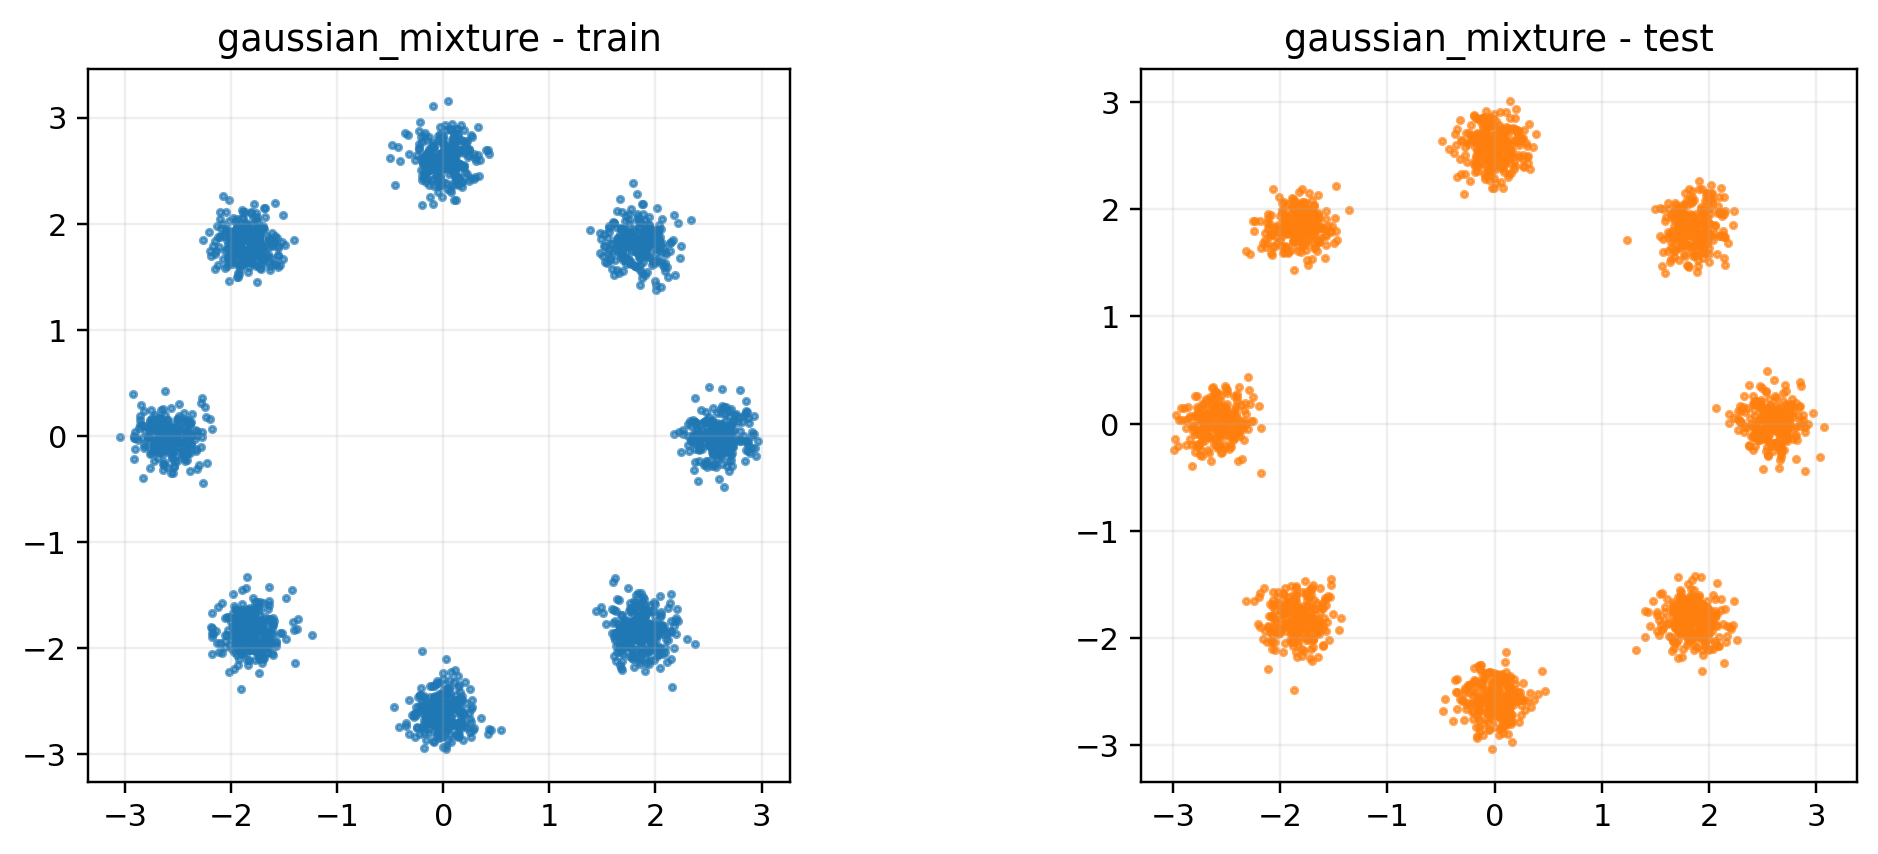
\includegraphics[width=\linewidth]{../outputs/figures/gaussian_mixture_dataset.png}
    \caption{Gaussian Mixture}
  \end{subfigure}
  \hfill
  \begin{subfigure}[b]{0.48\textwidth}
    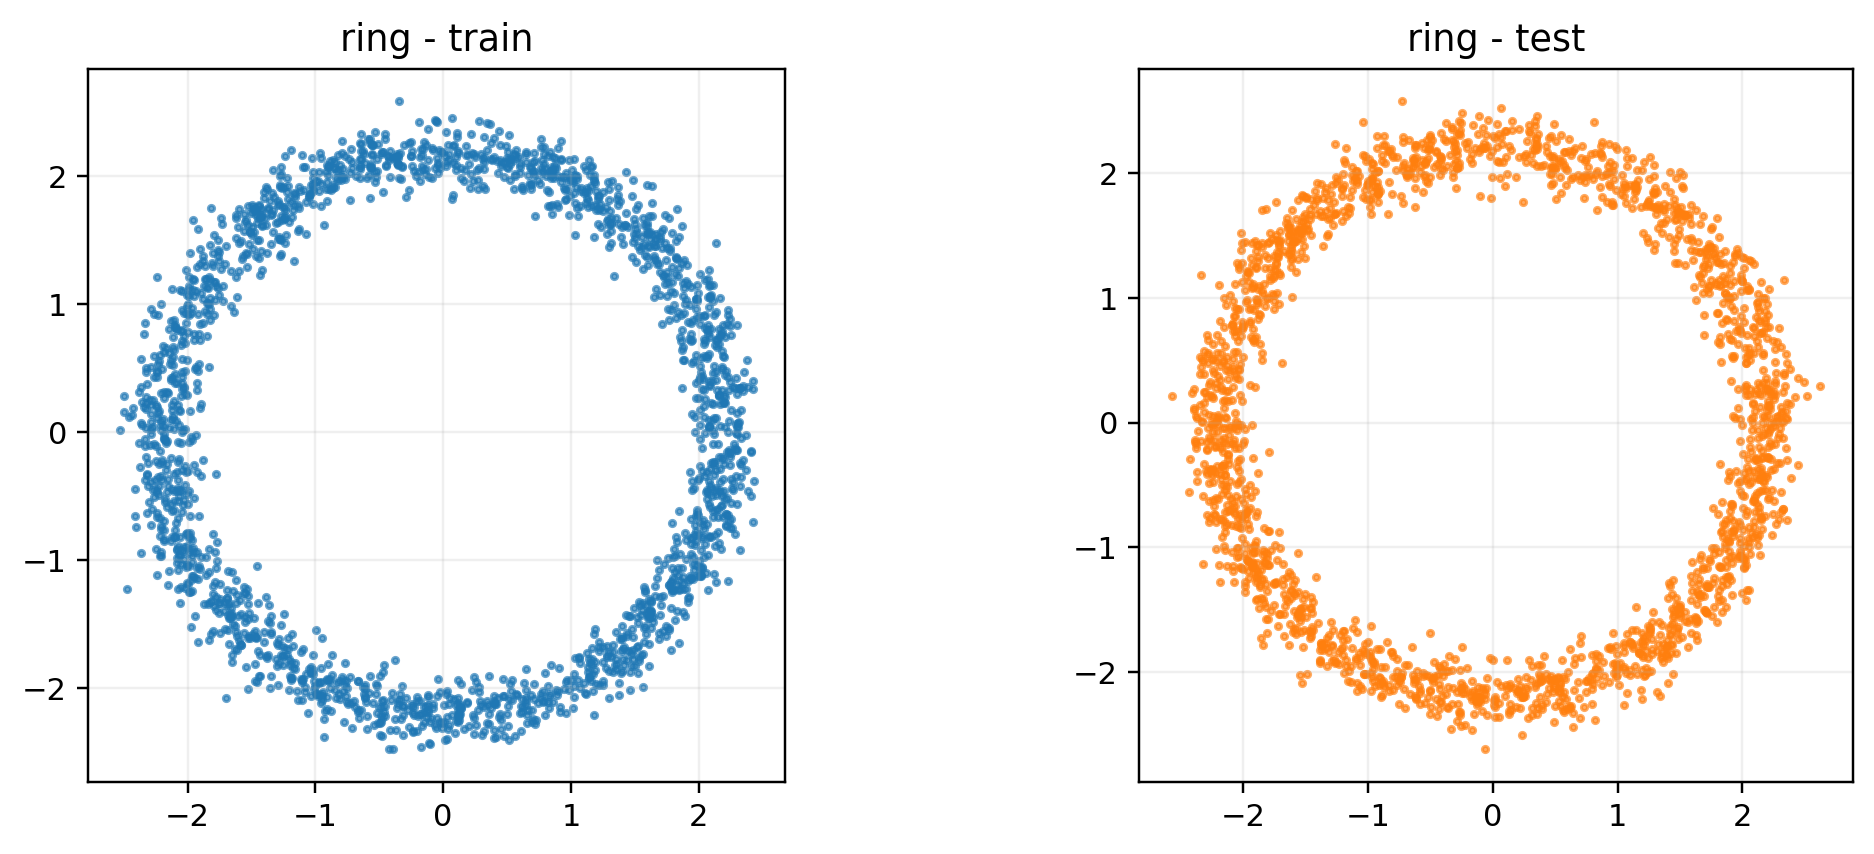
\includegraphics[width=\linewidth]{../outputs/figures/ring_dataset.png}
    \caption{Ring}
  \end{subfigure}
  \vspace{0.6em}
  \begin{subfigure}[b]{0.48\textwidth}
    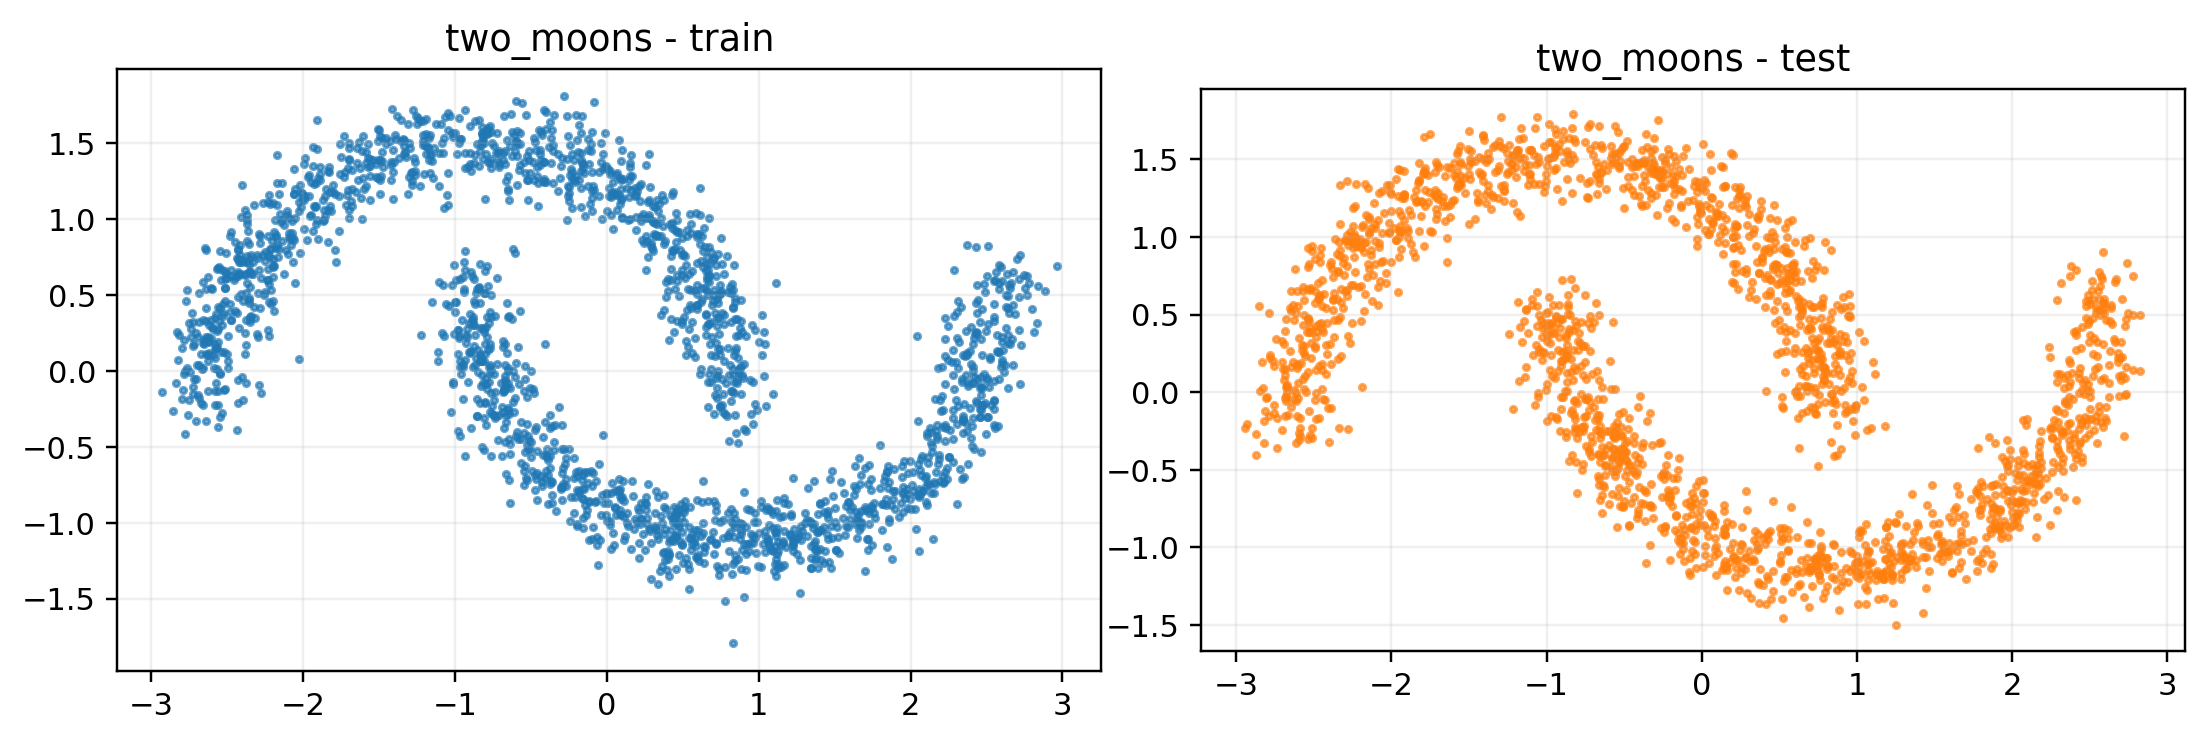
\includegraphics[width=\linewidth]{../outputs/figures/two_moons_dataset.png}
    \caption{Two Moons}
  \end{subfigure}
  \hfill
  \begin{subfigure}[b]{0.48\textwidth}
    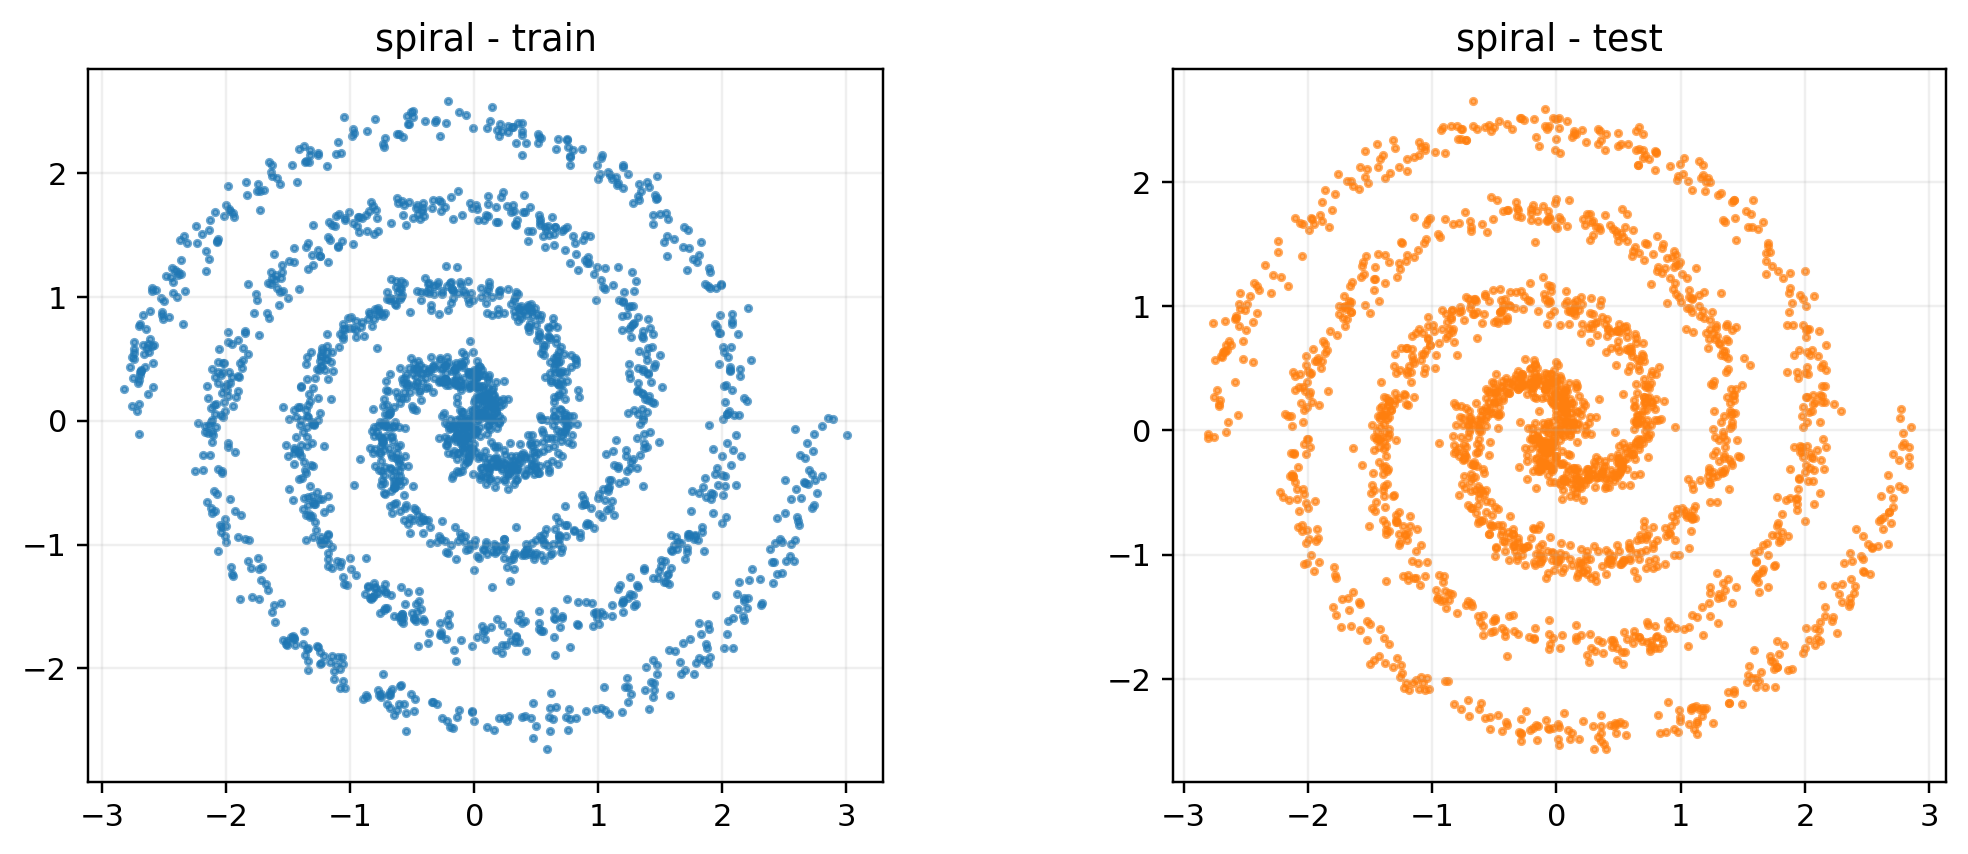
\includegraphics[width=\linewidth]{../outputs/figures/spiral_dataset.png}
    \caption{Spiral}
  \end{subfigure}
  \caption{统一数据格式下的四类二维分布。}
\end{figure}

\subsection{研究问题与本文结构}

为使实验与讨论形成清晰的闭环，本文将任务进一步凝练为以下三个研究问题：
\begin{enumerate}
  \item \textbf{RQ1：}在二维复杂分布生成任务中，VAE 与 Diffusion Model 分别具备怎样的分布拟合能力，它们在哪些分布类型上各自占优？
  \item \textbf{RQ2：}在生成质量、模式覆盖、几何结构保持与采样效率之间，两类模型存在怎样的权衡关系？
  \item \textbf{RQ3：}当关键超参数变化时，哪些因素会成为影响最终生成效果的主要控制变量？
\end{enumerate}

围绕上述问题，本文构建了统一的数据划分方式、训练协议、评价指标与可视化标准，并在相同实验条件下开展公平比较。全文后续结构如下：第二章综述相关工作；第三章给出模型假设与符号说明；第四章建立 VAE 与 Diffusion Model 的数学模型；第五章说明实验设计与实现细节；第六章给出结果分析与扩展实验；第七章总结主要结论并讨论两类模型的表现差异。

\section{相关工作}

\subsection{深度生成模型发展概述}

深度生成模型的发展大致经历了三个代表性阶段：早期的能量模型与概率图模型强调对联合分布的显式刻画，中期的 VAE 与 GAN 分别从变分推断和对抗学习两个方向推动了复杂数据生成研究，近年的扩散模型与流模型则进一步提升了样本质量与训练稳定性。不同范式的核心差异主要体现在三个方面：其一，模型如何表示数据分布；其二，训练时优化目标是否易于稳定求解；其三，采样阶段是一次性完成生成，还是通过多步迭代逐渐逼近目标分布。

\subsection{VAE 相关研究}

VAE 是深度生成模型中“显式潜变量建模”范式的代表方法，其奠基工作发表于 2014 年\cite{kingma2014vae}。这一框架的核心思想是：先用潜变量压缩样本的主要结构，再由解码器完成从潜空间到观测空间的重建，并通过重参数化技巧实现随机潜变量上的稳定反向传播。此类方法的优势在于理论结构清晰、训练过程稳定、潜空间具有较好的解释性；其局限则主要体现为样本容易出现过度平滑，对复杂局部几何形状的恢复能力相对有限。

\subsection{Diffusion Model 相关研究}

扩散模型是近年来深度生成领域的重要进展，DDPM 为这一方向奠定了标准化训练框架\cite{ho2020ddpm}。该方法利用前向加噪与反向去噪的对偶过程，把复杂分布生成问题拆解为一系列局部噪声预测子任务，因此在样本质量、训练稳定性和复杂结构表达方面都表现出较强能力。与 VAE 的“一步映射”不同，扩散模型体现的是“逐步逼近”思路：模型并不直接输出最终样本，而是从纯噪声开始，通过多次小幅修正逐渐恢复数据结构。其主要代价在于采样过程需要反复迭代，因此时间成本通常高于一次前向生成模型。

\subsection{分布一致性评价指标}

对于二维分布生成任务，相较于高维图像任务常依赖 FID 等间接指标，这里可以更直接地比较真实样本与生成样本的统计结构。本文采用三类互补指标：最大均值差异（MMD）用于刻画全局统计差异，切片 Wasserstein 距离（SWD）用于衡量几何形状一致性，Mode Coverage 用于分析多峰分布中的模式遗漏问题。相关定义和方法可参见文献\cite{gretton2012mmd}\allowbreak\cite{rabin2011swd}。这样的评价体系兼顾了全局统计差异、几何形状一致性以及模式完整性，能够较全面地反映二维点云生成质量。

\section{模型假设与符号说明}

\subsection{基本假设}

为保证两类模型比较具有可解释性，本文作如下统一假设：
\begin{enumerate}
  \item 训练集与测试集独立同分布抽样，且测试集能够代表目标分布；
  \item 两类模型均采用相同规模量级的 MLP 架构，避免由骨干网络容量造成系统性偏差；
  \item VAE 的潜变量先验与 Diffusion 的前向噪声均采用高斯分布假设；
  \item 所有实验在相同硬件环境、相同批量大小和相近优化策略下完成。
\end{enumerate}

\subsection{符号约定}

\begin{table}[H]
  \centering
  \caption{主要数学符号及其含义。}
  \begin{tabularx}{0.92\textwidth}{>{\centering\arraybackslash}p{0.18\textwidth} X X}
    \toprule
    符号 & 含义 & 说明 \\
    \midrule
    $x \in \R^2$ & 观测样本 & 二维坐标点 \\
    $z \in \R^d$ & 潜变量 & $d$ 为潜变量维度 \\
    $q_{\phi}(z|x)$ & 编码器近似后验 & $\phi$ 为编码器参数 \\
    $p_{\theta}(x|z)$ & 解码器条件分布 & $\theta$ 为解码器参数 \\
    $p(z)$ & 潜变量先验 & 通常取标准高斯 \\
    $T$ & 扩散步数 & DDPM 总时间步 \\
    $\beta_t,\bar{\alpha}_t$ & 噪声调度参数 & 控制加噪强度 \\
    $\epsilon_{\theta}(x_t,t)$ & 噪声预测网络 & 反向过程核心函数 \\
    MMD & 最大均值差异 & 分布整体一致性 \\
    SWD & 切片 Wasserstein 距离 & 几何搬运代价 \\
    \bottomrule
  \end{tabularx}
\end{table}

\subsection{四类分布的数学特征}

四类数据覆盖了典型的几何结构难点：
\begin{itemize}
  \item \textbf{Gaussian Mixture：}具有多模态结构，重点考察模型是否会发生模式丢失；
  \item \textbf{Ring：}样本集中于闭合低维流形附近，考察模型对薄环状结构的拟合能力；
  \item \textbf{Two Moons：}两条相互靠近但彼此分离的弯曲流形，考察局部几何保持能力；
  \item \textbf{Spiral：}连续螺旋结构最为复杂，考察模型对长程拓扑与全局连续性的学习能力。
\end{itemize}

\section{模型建立}

\subsection{变分自编码器}

\subsubsection{模型原理}

VAE 将样本生成过程表示为：先从先验分布 $p(z)$ 采样潜变量，再通过解码器 $p_{\theta}(x|z)$ 生成样本。对单个观测样本 $x$ 而言，其边际似然为
\begin{equation}
  p_{\theta}(x)=\int p_{\theta}(x|z)p(z)\,\mathrm{d}z
\end{equation}
直接对该积分求对数通常不可解析，因此引入近似后验 $q_{\phi}(z|x)$，并利用恒等变换
\begin{equation}
  \log p_{\theta}(x)
  =\log \int q_{\phi}(z|x)\frac{p_{\theta}(x,z)}{q_{\phi}(z|x)}\,\mathrm{d}z.
\end{equation}
由 Jensen 不等式可得证据下界（ELBO）
\begin{equation}
  \log p_{\theta}(x)\ge
  \mathbb{E}_{z\sim q_{\phi}(z|x)}[\log p_{\theta}(x|z)]
  -D_{\mathrm{KL}}(q_{\phi}(z|x)\|p(z)).
\end{equation}
进一步地，将联合分布写成 $p_{\theta}(x,z)=p_{\theta}(x|z)p(z)$，可得到更具解释性的分解
\begin{equation}
  \log p_{\theta}(x)
  =
  \underbrace{
  \mathbb{E}_{q_{\phi}(z|x)}[\log p_{\theta}(x|z)]
  -D_{\mathrm{KL}}(q_{\phi}(z|x)\|p(z))
  }_{\mathrm{ELBO}(x)}
  +
  D_{\mathrm{KL}}(q_{\phi}(z|x)\|p_{\theta}(z|x)).
\end{equation}
由于最后一项 KL 散度非负，最大化 ELBO 等价于同时推动两个目标：一方面提高重构项 $\mathbb{E}_{q_{\phi}(z|x)}[\log p_{\theta}(x|z)]$，使解码后的样本尽可能接近原样本；另一方面约束近似后验 $q_{\phi}(z|x)$ 不要偏离先验 $p(z)$ 太远，从而使潜空间保持规整、可采样。

在实际实现中，本文采用均方误差近似重构项，并在 KL 散度前加入可调权重 $\beta$，得到训练目标
\begin{equation}
  \mathcal{L}_{\mathrm{VAE}}=
  \mathbb{E}_{x\sim p_{\mathrm{data}}}
  \left[\|x-\hat{x}\|_2^2+\beta D_{\mathrm{KL}}(q_{\phi}(z|x)\|p(z))\right].
\end{equation}
当 $q_{\phi}(z|x)$ 取对角高斯分布
\begin{equation}
  q_{\phi}(z|x)=\Ncal(\mu_{\phi}(x),\mathrm{diag}(\sigma_{\phi}^2(x))),
\end{equation}
且先验取标准高斯 $p(z)=\Ncal(0,I)$ 时，KL 项可以写成闭式形式
\begin{equation}
  D_{\mathrm{KL}}(q_{\phi}(z|x)\|p(z))
  =
  \frac{1}{2}\sum_{k=1}^{d}
  \left(
  \mu_k^2+\sigma_k^2-\log \sigma_k^2-1
  \right).
\end{equation}
这一表达式清楚说明：若某个潜变量维度的均值过大、方差过大或方差过小，都会带来额外惩罚，因此 KL 项本质上在控制潜空间分布向标准高斯靠拢。

\subsubsection{重参数化技巧}

为使随机采样过程可微，采用重参数化技巧
\begin{equation}
  z=\mu_{\phi}(x)+\sigma_{\phi}(x)\odot\epsilon,\qquad \epsilon\sim\Ncal(0,I),
\end{equation}
其中 $\mu_{\phi}(x)$ 与 $\log\sigma_{\phi}^2(x)$ 由编码器输出。该技巧的关键在于：原本对随机变量 $z\sim q_{\phi}(z|x)$ 的采样，被改写为对与参数无关的外部噪声 $\epsilon$ 进行采样，再通过确定性函数映射得到 $z$。于是期望项
\begin{equation}
  \mathbb{E}_{z\sim q_{\phi}(z|x)}[f(z)]
\end{equation}
可转化为
\begin{equation}
  \mathbb{E}_{\epsilon\sim\Ncal(0,I)}
  \bigl[f(\mu_{\phi}(x)+\sigma_{\phi}(x)\odot\epsilon)\bigr],
\end{equation}
从而允许梯度直接传播到 $\mu_{\phi}(x)$ 和 $\sigma_{\phi}(x)$，这正是 VAE 能够以标准反向传播方式训练的关键。

\subsubsection{网络结构}

本文 VAE 采用轻量级 MLP 架构：输入为二维坐标，编码器和解码器均为两层 128 维隐藏层，潜变量维度设为 4，优化器使用 Adam，学习率为 $10^{-3}$，主实验训练 150 个 epoch，批量大小为 256。选择 $d=4$ 的原因在于其既能为复杂分布提供足够表示容量，又不会使低维潜空间的可解释性显著下降。

\subsection{扩散概率模型}

\subsubsection{前向扩散过程}

扩散模型的前向过程是一条马尔可夫链，在每个时间步中向样本注入少量高斯噪声：
\begin{equation}
  q(x_t|x_{t-1})=\Ncal\left(\sqrt{1-\beta_t}\,x_{t-1},\,\beta_t I\right).
\end{equation}
利用高斯分布的封闭性，可直接写出任意时刻相对于原始样本 $x_0$ 的边际分布：
\begin{equation}
  x_t=\sqrt{\bar{\alpha}_t}\,x_0+\sqrt{1-\bar{\alpha}_t}\,\epsilon,\qquad \epsilon\sim\Ncal(0,I),
\end{equation}
其中 $\alpha_t=1-\beta_t$，$\bar{\alpha}_t=\prod_{s=1}^{t}\alpha_s$。该公式表明：任意时刻的带噪样本都可以理解为“原始样本 $x_0$ 的缩放版本”与“标准高斯噪声”的线性组合。随着 $t$ 增大，$\bar{\alpha}_t$ 逐渐减小，原始数据结构的占比持续下降，噪声占比持续上升，最终使分布逐步逼近标准高斯。

\subsubsection{反向去噪过程}

若已知 $x_0$，则根据高斯条件分布的性质，可以写出单步反向后验
\begin{equation}
  q(x_{t-1}\mid x_t,x_0)=
  \Ncal\bigl(x_{t-1};\tilde{\mu}_t(x_t,x_0),\tilde{\beta}_t I\bigr),
\end{equation}
其中
\begin{equation}
  \tilde{\mu}_t(x_t,x_0)
  =
  \frac{\sqrt{\bar{\alpha}_{t-1}}\beta_t}{1-\bar{\alpha}_t}x_0
  +
  \frac{\sqrt{\alpha_t}(1-\bar{\alpha}_{t-1})}{1-\bar{\alpha}_t}x_t,
\end{equation}
\begin{equation}
  \tilde{\beta}_t=
  \frac{1-\bar{\alpha}_{t-1}}{1-\bar{\alpha}_t}\beta_t.
\end{equation}
真正困难之处在于采样阶段并不知道真实的 $x_0$。因此 DDPM 不直接学习 $x_{t-1}$ 或 $x_0$，而是训练一个噪声预测网络 $\epsilon_{\theta}(x_t,t)$ 来估计前向过程中加入的噪声。根据
\begin{equation}
  x_t=\sqrt{\bar{\alpha}_t}x_0+\sqrt{1-\bar{\alpha}_t}\epsilon,
\end{equation}
可将 $x_0$ 估计为
\begin{equation}
  \hat{x}_0(x_t,t)=
  \frac{1}{\sqrt{\bar{\alpha}_t}}
  \left(
  x_t-\sqrt{1-\bar{\alpha}_t}\,\epsilon_{\theta}(x_t,t)
  \right).
\end{equation}
再将其代回反向均值公式，即可得到模型对 $p_{\theta}(x_{t-1}\mid x_t)$ 的近似。Ho 等人的 DDPM 进一步证明，在固定方差设定下，原始变分下界可以化简为噪声预测形式的均方误差目标
\begin{equation}
  \mathcal{L}_{\mathrm{diffusion}}=
  \mathbb{E}_{x_0,\epsilon,t}\left[\|\epsilon-\epsilon_{\theta}(x_t,t)\|_2^2\right].
\end{equation}
在采样阶段，模型从纯噪声 $x_T\sim\Ncal(0,I)$ 出发，逐步执行 $T,T-1,\dots,1$ 的反向迭代，持续利用当前样本与时间步估计噪声，再据此修正样本位置，最终恢复出近似服从目标分布的样本。与 VAE 的单步解码相比，这一过程将复杂生成任务拆解为多个局部去噪子任务，因此在几何结构保真度上往往更具优势。

\subsubsection{噪声调度与网络配置}

本文采用线性噪声调度，设置 $\beta_{\mathrm{start}}=10^{-4}$、$\beta_{\mathrm{end}}=0.02$，主实验步数为 $T=80$。噪声预测网络为三层 MLP，时间步信息通过正弦位置编码嵌入后与输入拼接，以便模型在不同去噪阶段学习不同策略。与 VAE 相比，Diffusion Model 的优势在于分步建模降低了单次映射难度，代价则是采样必须执行多轮前向推理。

\subsection{评价指标体系}

\subsubsection{最大均值差异}

对于真实样本集合 $X=\{x_i\}_{i=1}^{m}$ 与生成样本集合 $Y=\{y_j\}_{j=1}^{n}$，MMD 的无偏估计可写为
\begin{equation}
  \mathrm{MMD}^2(X,Y)=
  \frac{1}{m^2}\sum_{i,j}k(x_i,x_j)
  +\frac{1}{n^2}\sum_{i,j}k(y_i,y_j)
  -\frac{2}{mn}\sum_{i,j}k(x_i,y_j),
\end{equation}
其中核函数采用 RBF 核。MMD 越小，说明两组样本在整体统计意义上越接近。该指标的优势在于能够直接在样本层面比较两组分布，无需显式密度估计；其局限在于结果会受到核函数形式与带宽参数选择的影响，而且对局部几何细节的敏感性通常不如 Wasserstein 类距离。

\subsubsection{切片 Wasserstein 距离}

设 $\theta \in \mathbb{S}^{1}$ 表示单位圆上的一个投影方向，$P_{\theta}(x)=\langle \theta,x\rangle$ 表示样本在该方向上的一维投影，则切片 Wasserstein 距离可写为
\begin{equation}
  \mathrm{SWD}(X,Y)=
  \mathbb{E}_{\theta\sim \mathrm{Unif}(\mathbb{S}^{1})}
  \Big[
    W_1\big(P_{\theta}\sharp \mu_X,\; P_{\theta}\sharp \mu_Y\big)
  \Big],
\end{equation}
其中 $\mu_X,\mu_Y$ 分别表示真实样本与生成样本的经验分布，$P_{\theta}\sharp \mu$ 表示测度在方向 $\theta$ 下的推前分布。实际计算中，本文采用有限个随机方向对该期望进行 Monte Carlo 近似。SWD 通过将二维点云投影到多个随机一维方向上，再分别计算一维 Wasserstein 距离并求平均，从而在保持几何敏感性的同时降低计算成本。SWD 越小，表明生成分布在几何形状和空间位移上越接近真实分布。其局限在于：投影方向数量不足时结果可能存在随机波动，而且不同方向上的一维投影会压缩原始高维几何信息，因此它反映的是“平均投影意义下”的几何接近程度，而非完整几何结构的一一对应。

\subsubsection{模式覆盖率}

对于多峰分布，仅依靠 MMD 或 SWD 仍可能掩盖模式坍塌问题。为此，本文先对真实测试集进行聚类，设聚类总数为 $K$，若生成样本在第 $k$ 个聚类邻域中出现的样本数不少于预设阈值，则记该模态被成功覆盖。于是模式覆盖率定义为
\begin{equation}
  \mathrm{Coverage}=
  \frac{1}{K}\sum_{k=1}^{K}\mathbf{1}\!\left(n_k^{(\mathrm{gen})}\ge \tau\right),
\end{equation}
其中 $n_k^{(\mathrm{gen})}$ 表示落入第 $k$ 个真实模态邻域的生成样本数，$\tau$ 为覆盖判定阈值。Coverage 越接近 1，说明生成样本越不容易遗漏真实分布中的主要模态。对于 Gaussian Mixture，该指标尤其具有解释力；对于 Ring 与 Spiral，它更多用于补充分析而非单独决策。其局限在于：结果依赖于聚类数目、邻域划分方式和阈值设定，而且它只能反映“是否覆盖到某个模态”，不能直接衡量模态内部的密度形状、边界精度与局部几何质量。

\section{实验设计与数值方法}

\subsection{数据生成与预处理}

本文直接采用统一的数组式数据组织方式生成四类二维分布，并划分为训练集、测试集和隐藏测试集。公开实验仅使用训练/测试部分，所有样本通过统一标签完成分布切片，避免在训练和评价阶段重复数据转换。数据组织与模型训练过程相互独立，使得后续若数据来源发生变化，只需替换底层数据文件而无需重写建模与评价流程。

除基础散点图外，本文还对四类分布进行描述性统计分析，以便更系统地理解它们的几何差异。表 \ref{tab:data-summary} 汇总了训练集的代表性统计量。可以看出，Gaussian Mixture 具有最大的协方差迹（约 6.84），对应明显分离的多模态结构；Ring 的平均半径约为 2.20 且标准差很小，说明样本主要集中于一条窄环带；Two Moons 的半径均值约 2.05 但标准差达到 0.84，体现出其非均匀弯曲流形的几何复杂性；Spiral 的协方差迹和平均半径均较小，但由于其点集沿连续螺旋线展开，长程结构学习仍然最具挑战性。

\begin{table}[H]
  \centering
  \caption{四类训练集的描述性统计量。}
  \label{tab:data-summary}
  \begin{tabular}{lcccccc}
    \toprule
    数据集 & $\mu_x$ & $\mu_y$ & $\sigma_x$ & $\sigma_y$ & 平均半径 & 协方差迹 \\
    \midrule
    Gaussian Mixture & -0.013 & 0.013 & 1.809 & 1.886 & 2.607 & 6.844 \\
    Ring             & -0.023 & -0.108 & 1.554 & 1.551 & 2.195 & 4.831 \\
    Two Moons        & 0.000 & 0.000 & 1.918 & 1.107 & 2.051 & 4.913 \\
    Spiral           & 0.158 & 0.209 & 1.133 & 1.211 & 1.460 & 2.755 \\
    \bottomrule
  \end{tabular}
\end{table}

从建模难度上看，四类分布形成了一个较清晰的难度阶梯：Gaussian Mixture 主要考察模式覆盖；Ring 重点考察低维闭合流形的保形能力；Two Moons 强调局部间隔与流形弯曲的兼顾；Spiral 则同时要求全局拓扑连续性、局部噪声鲁棒性以及长程结构一致性，因此在整个实验中被视为最具代表性的“压力测试”数据集。

\subsection{训练流程}

VAE 的训练以重构项与 KL 项之和为优化目标；Diffusion Model 的训练则通过随机时间步上的噪声预测误差完成参数更新。两类模型均采用 Adam 优化器与相近的批量大小，因此训练耗时具有较强可比性。

为使实验部分更具层次性，本文将全部实验划分为三层：
\begin{enumerate}
  \item \textbf{主实验层：}针对四类分布分别训练 VAE 与 Diffusion Model，共 8 组核心实验；
  \item \textbf{超参数分析层：}围绕 VAE 的 KL 权重和 Diffusion 的扩散步数开展消融实验；
  \item \textbf{拓展实验层：}增加骨干增强、采样加速、条件扩散、多类型污染鲁棒性与高维 lifted 验证，以补充对模型能力边界的考察。
\end{enumerate}

这种“主实验 + 消融 + 拓展分析”的三层结构，使正文能够先给出主结论，再通过更细的对照实验解释结论来源，最后补充模型设计与分析深度。

\subsection{实现环境与可复现性}

全部实验在统一的软件与硬件环境下完成，VAE 与 Diffusion Model 共享相同的数据切分、随机种子控制、评价指标定义与可视化规范，从而使结果差异尽可能反映模型机理本身，而非外部实现条件。

实验设备配备 NVIDIA GeForce RTX 5060 Laptop GPU。对于二维任务而言，这一配置足以支持主实验、消融实验、条件生成与鲁棒性分析的系统比较。二维实验并不追求复现高维图像任务的绝对计算成本，而是利用较低资源门槛换取更密集的对照实验，使模型差异能够在统一协议下被更清楚地识别和解释。

\section{实验结果与分析}

\subsection{训练过程分析}

\begin{figure}[H]
  \centering
  \begin{subfigure}[b]{0.48\textwidth}
    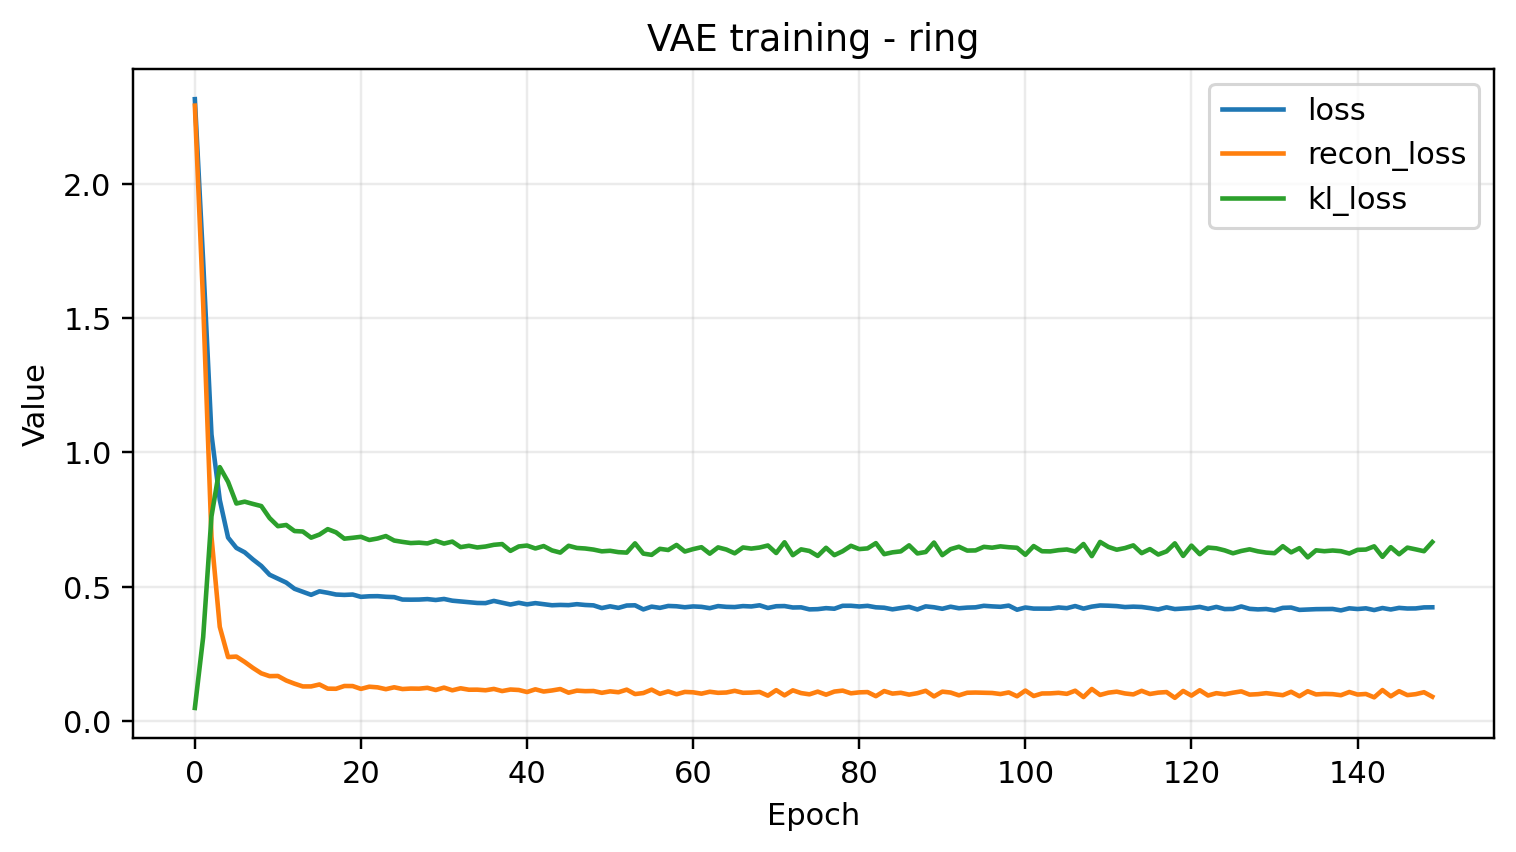
\includegraphics[width=\linewidth]{../outputs/figures/vae_ring_training.png}
    \caption{VAE on Ring}
  \end{subfigure}
  \hfill
  \begin{subfigure}[b]{0.48\textwidth}
    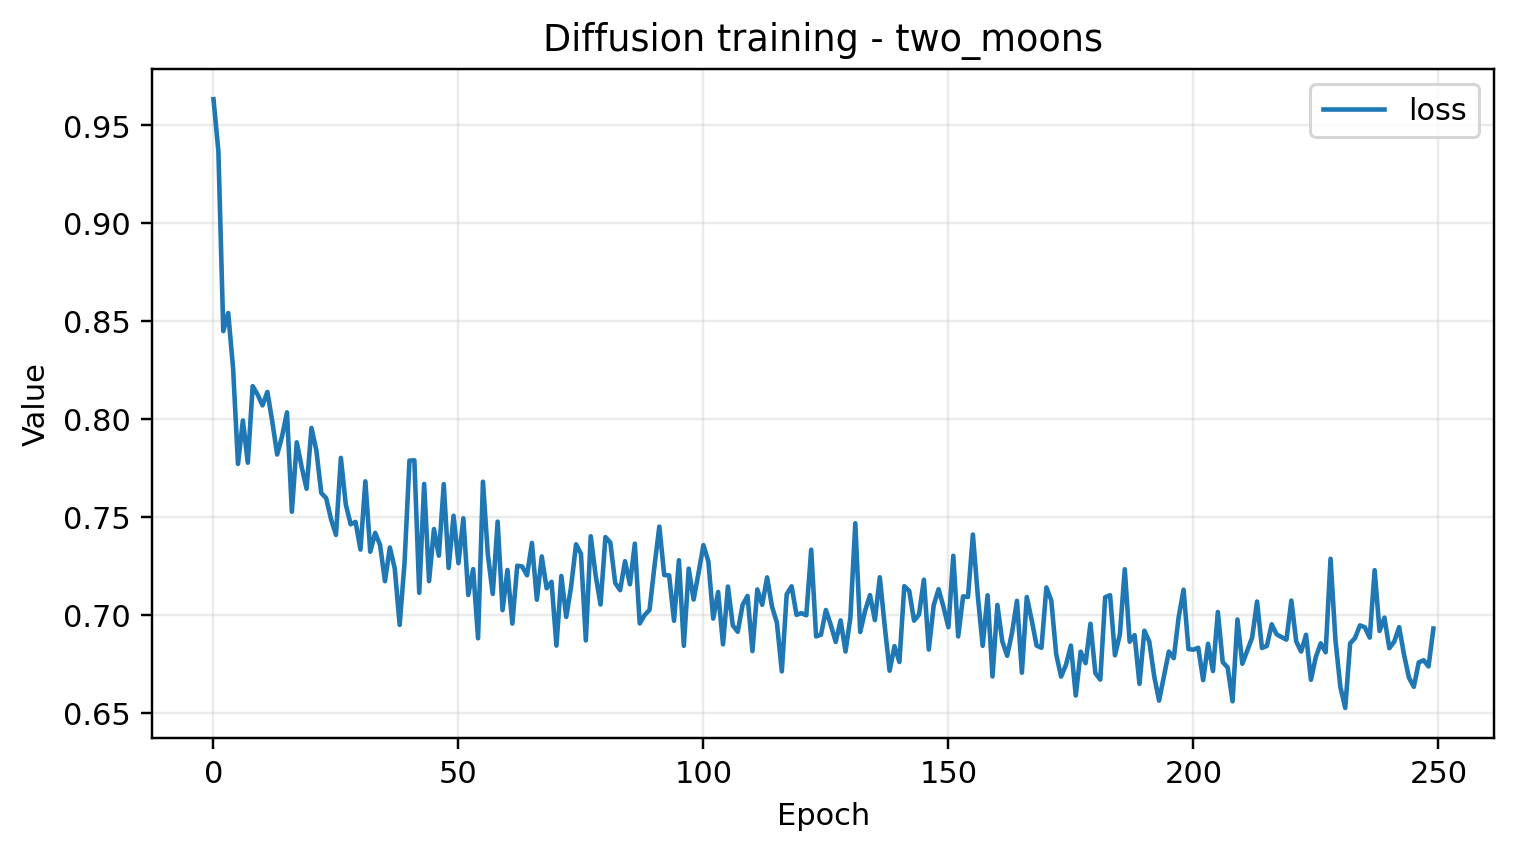
\includegraphics[width=\linewidth]{../outputs/figures/diffusion_two_moons_training.png}
    \caption{Diffusion on Two Moons}
  \end{subfigure}
  \caption{代表性训练曲线。VAE 的重构项快速下降后趋于平稳，Diffusion 的噪声预测损失在约 100--150 个 epoch 后进入收敛区间。}
\end{figure}

从训练曲线可以观察到，两类模型的优化过程均较为稳定。VAE 的训练动力学表现为重构损失快速下降、KL 项逐渐上升后稳定；Diffusion Model 的噪声预测均方误差则呈单调下降趋势。由于当前任务仅为二维分布拟合，二者在训练时间上的差异并不显著，主要差别集中在采样阶段。

这一现象说明，“训练是否稳定”并不是两类方法的关键分野，真正的差异来自模型如何组织生成过程。VAE 将全部结构恢复任务压缩到一次解码中，因此其采样极快但更容易平滑化；Diffusion 通过多个去噪步骤分担生成难度，因此样本质量较高但推理速度显著更慢。换言之，二维任务虽然形式简单，却已经足以暴露两种生成范式最本质的结构性差异。

\subsection{主实验定量结果}

\begin{table}[H]
  \centering
  \caption{VAE 与 Diffusion Model 在四类分布上的主实验结果。}
  \small
  \begin{tabular}{llccccc}
    \toprule
    模型 & 数据集 & MMD & SWD & Mode Cov. & 训练时间/s & 采样时间/s \\
    \midrule
    Diffusion & Gaussian Mixture & 0.0017 & 0.1414 & 1.00 & 4.1762 & 0.0407 \\
    VAE       & Gaussian Mixture & 0.0015 & 0.1732 & 1.00 & 3.5826 & 0.0012 \\
    Diffusion & Ring             & 0.0008 & 0.0909 & 1.00 & 3.9372 & 0.0393 \\
    VAE       & Ring             & 0.0019 & 0.1177 & 1.00 & 3.1983 & 0.0004 \\
    Diffusion & Spiral           & 0.0008 & 0.0683 & 1.00 & 3.9865 & 0.0397 \\
    VAE       & Spiral           & 0.0015 & 0.0747 & 1.00 & 3.2380 & 0.0004 \\
    Diffusion & Two Moons        & 0.0057 & 0.1450 & 1.00 & 4.1701 & 0.0367 \\
    VAE       & Two Moons        & 0.0017 & 0.1041 & 1.00 & 3.3577 & 0.0003 \\
    \bottomrule
  \end{tabular}
\end{table}

表中结果表明：在统一数据格式下，Diffusion Model 在 Ring 与 Spiral 上均取得更低的 MMD 与 SWD，说明其在闭合流形和连续螺旋这类复杂几何结构上的恢复能力更强；VAE 在 Gaussian Mixture 与 Two Moons 上的 MMD 更低，表明对于多峰但边界清晰、或局部连续性较强的分布，单步生成模型依然具有较强拟合能力。值得注意的是，两类模型的训练时间仍处于同一量级，但采样时间相差约两个数量级，这一结果与两种模型的生成机制完全一致。

进一步看，主实验中的差异具有明确的结构指向。其一，Diffusion Model 的优势主要集中在 Ring 与 Spiral 这类需要维持全局连续几何的分布上，这与其逐步去噪的生成机制一致。其二，VAE 在 Gaussian Mixture 与 Two Moons 上取得更低的 MMD，并在采样效率上保持显著优势，说明单步生成模型在边界清晰或局部连续性较强的分布上仍具有较强竞争力。其三，Mode Coverage 在全部主实验中均达到 1.0，说明当前实验设置下两类模型都能覆盖主要模态，性能差异主要来自几何保真度而非模式遗漏。

\subsection{分布别结果讨论}

为了更清晰地呈现不同分布结构下的性能差异，下面按数据集逐一讨论两类模型的表现。

\textbf{Gaussian Mixture：}该分布由多个相互分离的局部高斯团簇组成，主要难点在于同时覆盖多个模态，并保持各模态位置与方差尺度的一致性。本次重跑中 VAE 的 MMD 为 0.0015，略优于 Diffusion 的 0.0017，但 Diffusion 在 SWD 上更低（0.1414 vs 0.1732），说明二者都能覆盖多峰结构，而 Diffusion 在几何搬运意义下的整体对齐更稳定。

\textbf{Ring：}Ring 分布本质上是一条一维闭合流形嵌入二维平面的问题，因此模型需要尽量避免将窄环“涂厚”或“填实”。Diffusion Model 在该分布上的 MMD 和 SWD 分别达到 0.0008 与 0.0909，均显著优于 VAE 的 0.0019 与 0.1177，表明它更善于恢复细薄环带；VAE 则更容易生成厚度偏大的环形点云，这是一种典型的均值化效应。

\textbf{Two Moons：}Two Moons 是主实验中最“反例化”的一个数据集。VAE 在 MMD 上明显优于 Diffusion（0.0017 vs 0.0057），且 SWD 也更低（0.1041 vs 0.1450），说明对于局部连续但整体拓扑并不太复杂的双月流形，显式潜变量建模并不一定处于劣势，反而能够更紧地贴合真实流形。

\textbf{Spiral：}Spiral 是四类分布中最具挑战性的对象。Diffusion Model 在主实验中以 0.0008 的 MMD 和 0.0683 的 SWD 优于 VAE 的 0.0015 和 0.0747，且结合图像可见其螺旋连续性更好。对于这一类需要兼顾长程连续性和局部噪声鲁棒性的结构，Diffusion 更容易逐步“雕刻”出全局形状，而 VAE 更容易在局部产生平滑化或断裂。

\subsection{定性可视化分析}

\begin{figure}[H]
  \centering
  \begin{subfigure}[b]{0.48\textwidth}
    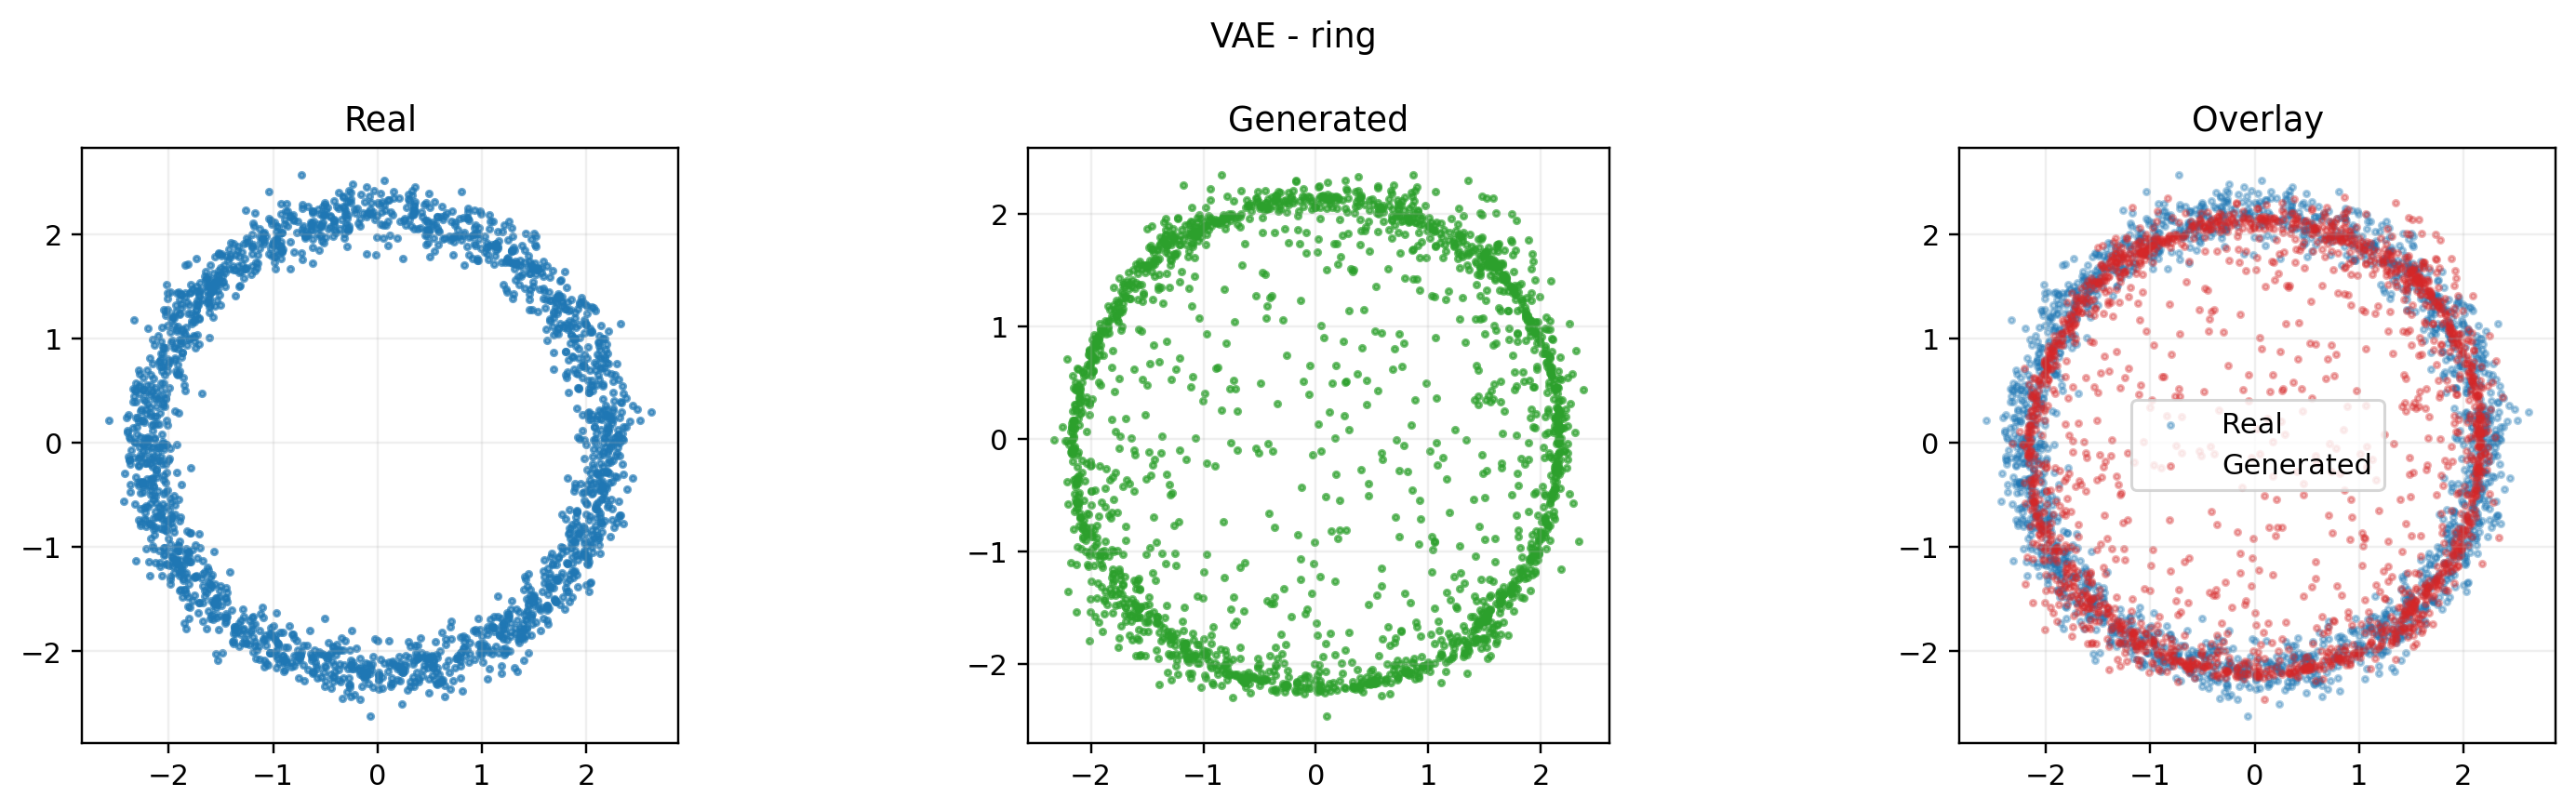
\includegraphics[width=\linewidth]{../outputs/figures/vae_ring_samples.png}
    \caption{VAE on Ring}
  \end{subfigure}
  \hfill
  \begin{subfigure}[b]{0.48\textwidth}
    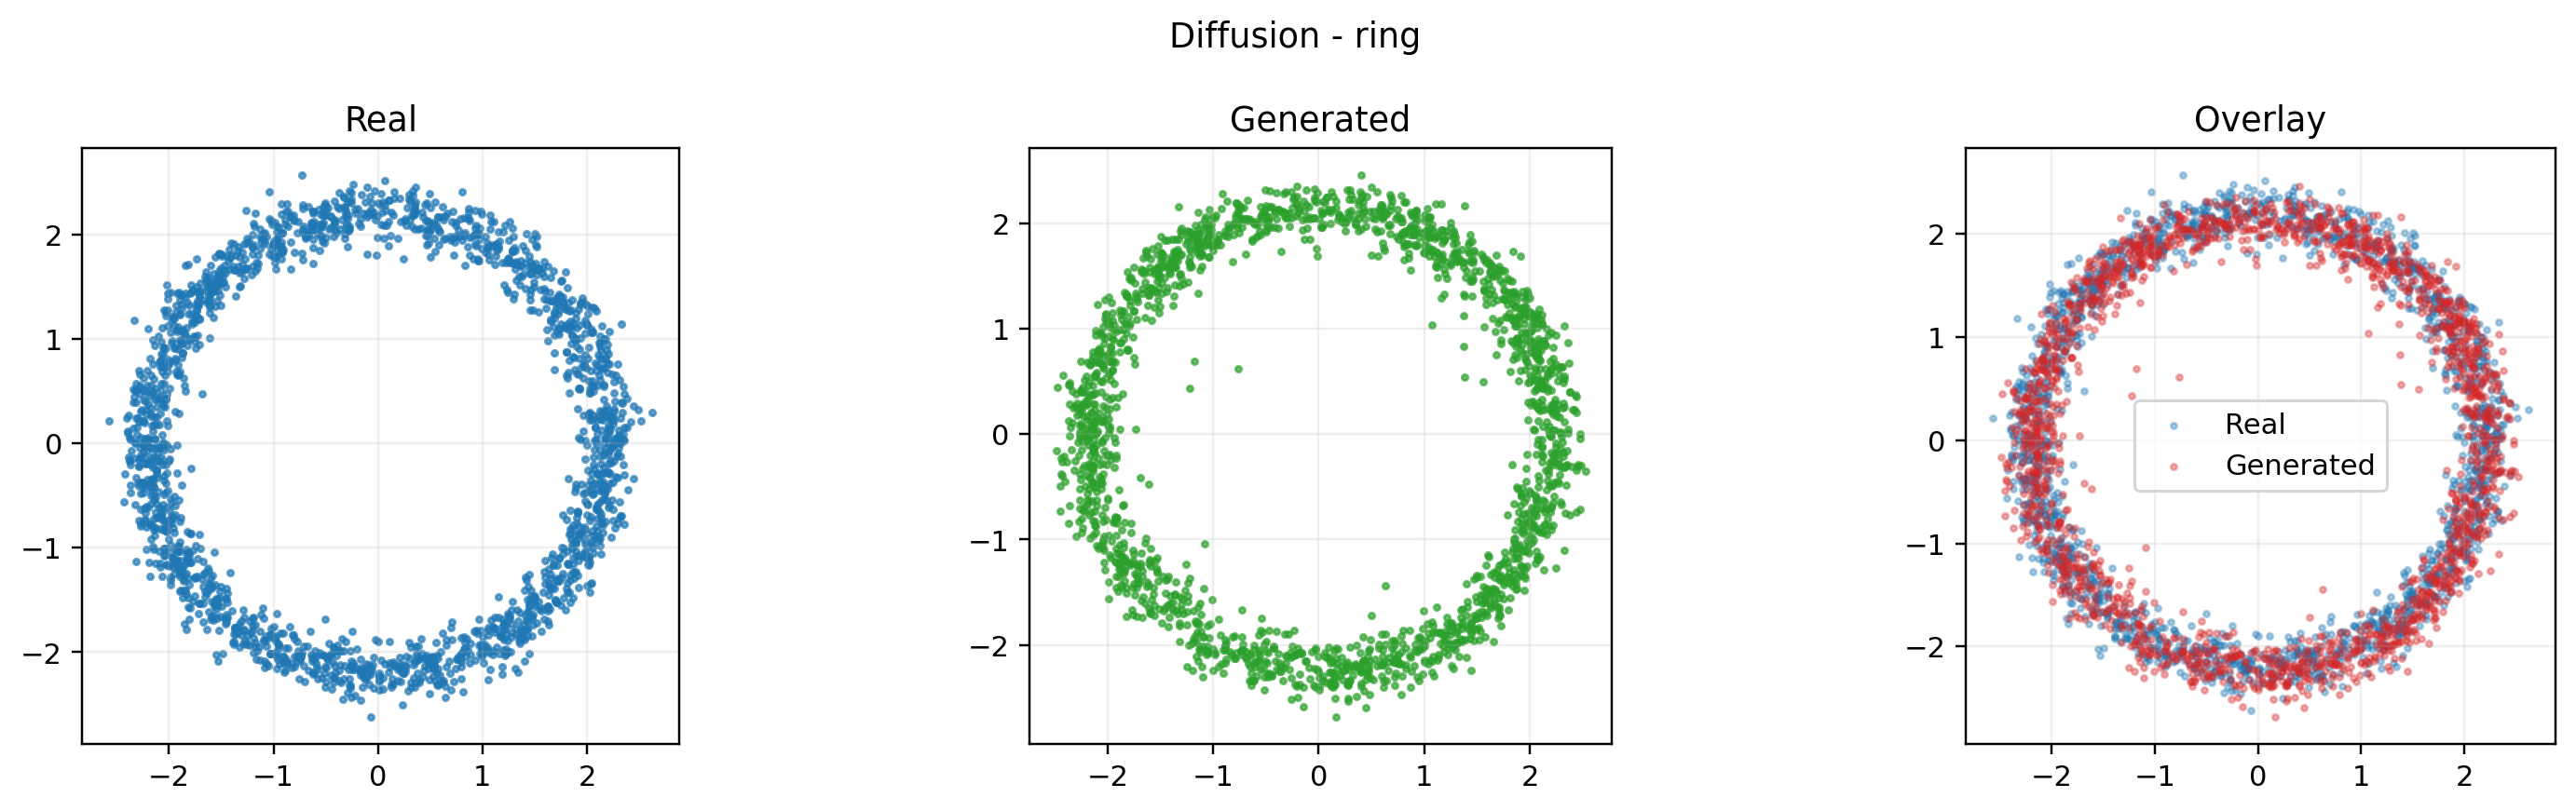
\includegraphics[width=\linewidth]{../outputs/figures/diffusion_ring_samples.png}
    \caption{Diffusion on Ring}
  \end{subfigure}
  \vspace{0.6em}
  \begin{subfigure}[b]{0.48\textwidth}
    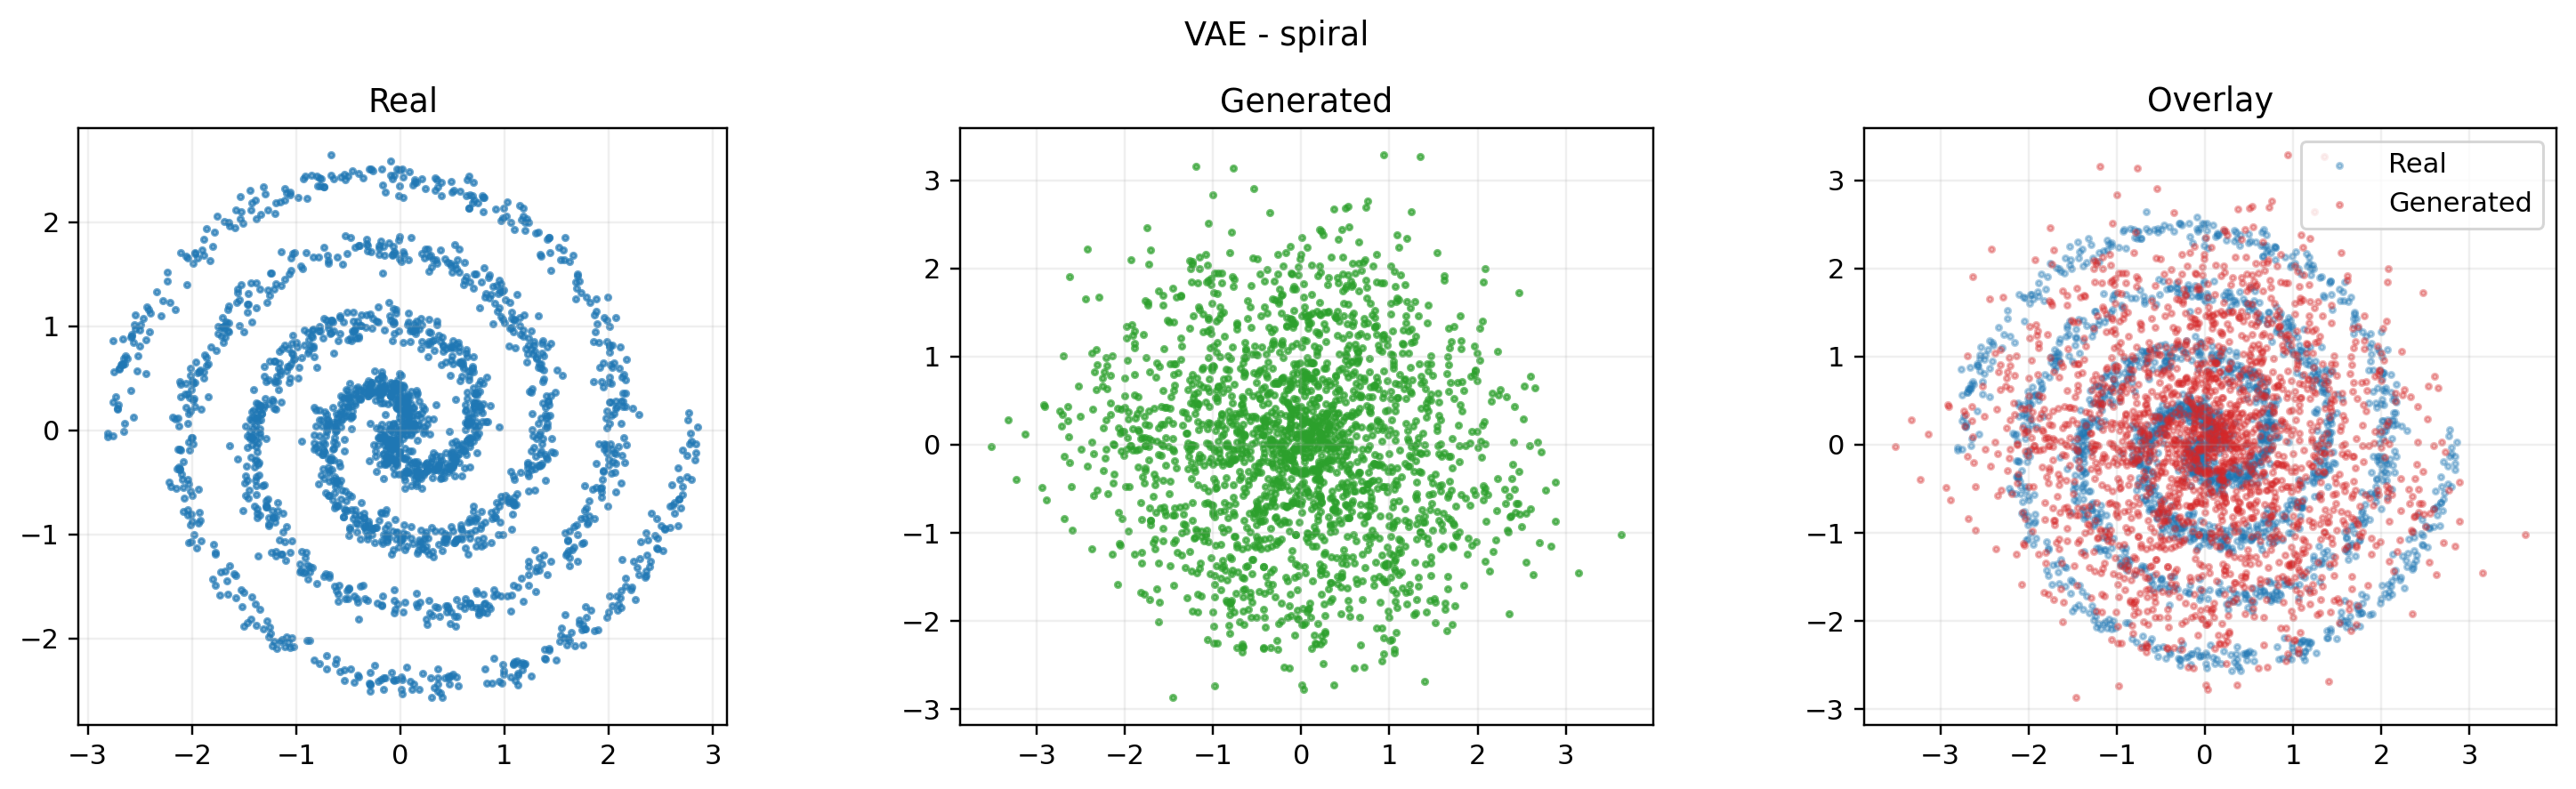
\includegraphics[width=\linewidth]{../outputs/figures/vae_spiral_samples.png}
    \caption{VAE on Spiral}
  \end{subfigure}
  \hfill
  \begin{subfigure}[b]{0.48\textwidth}
    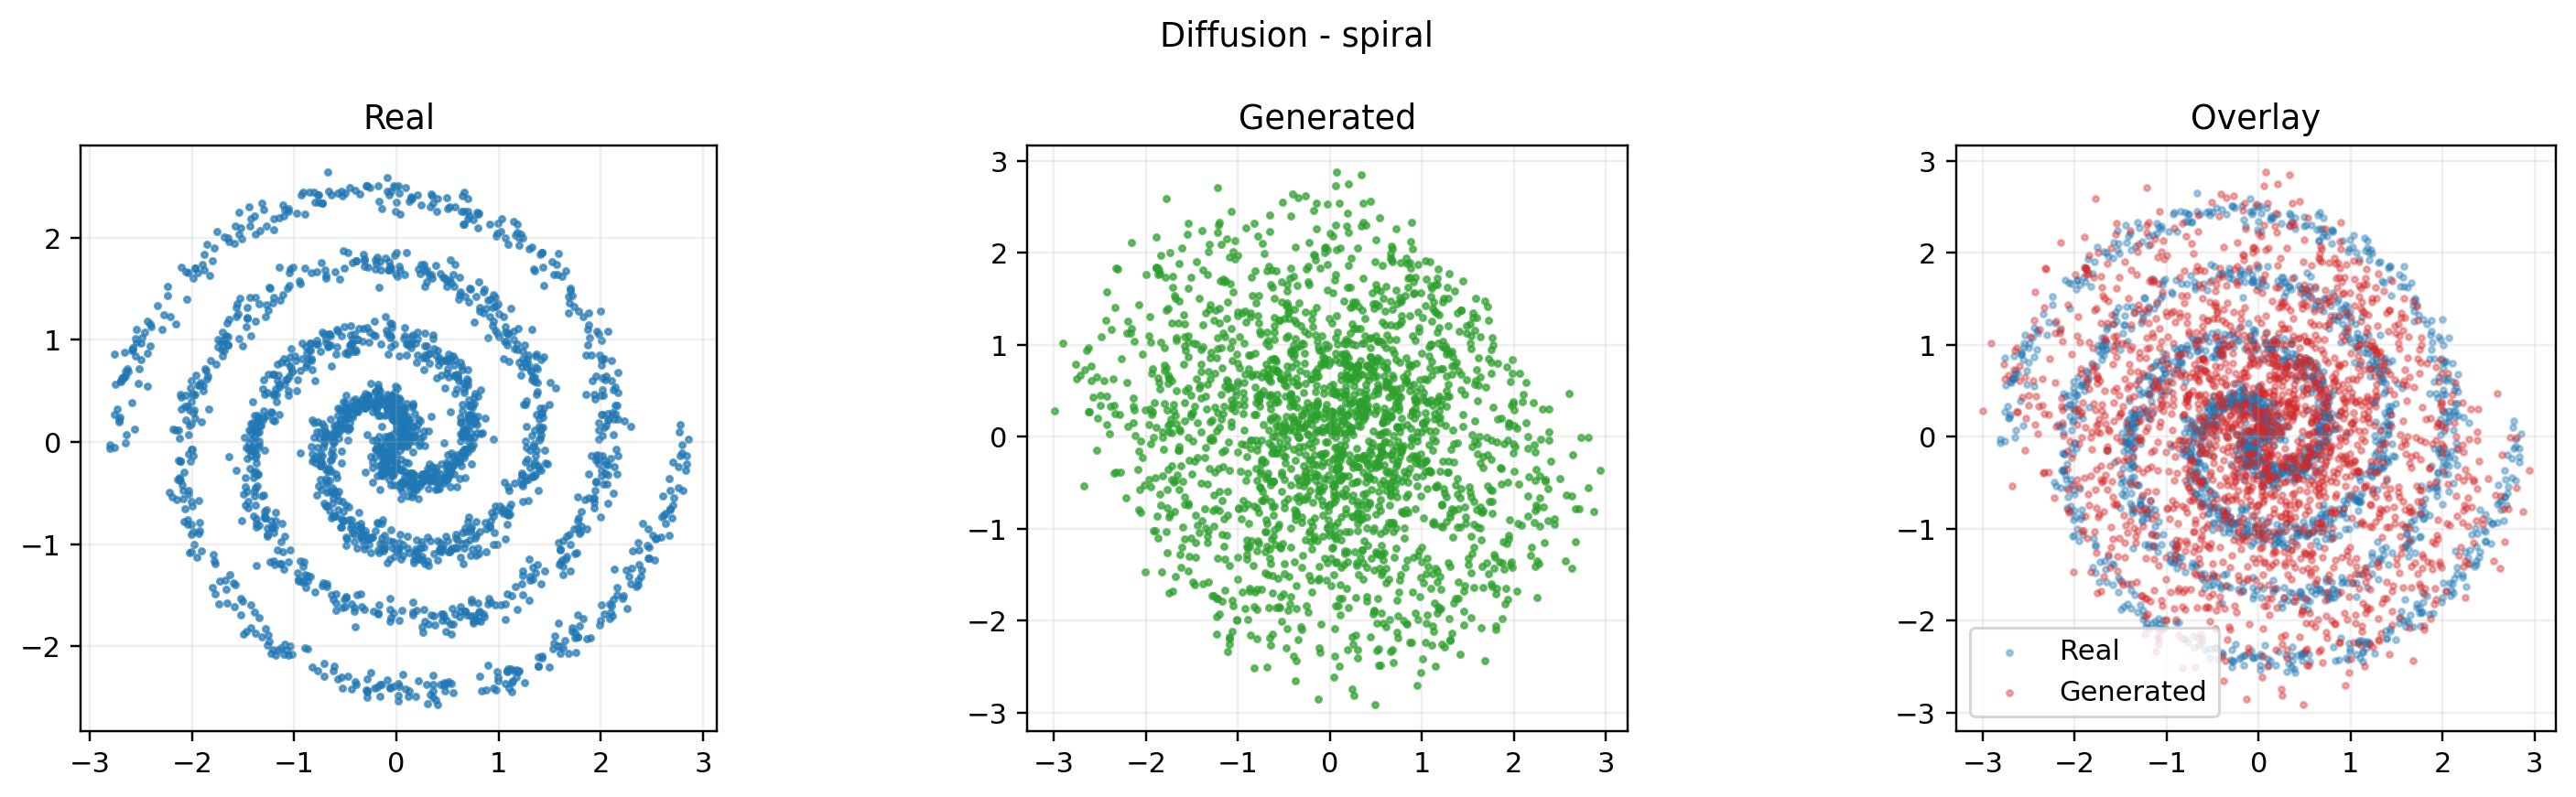
\includegraphics[width=\linewidth]{../outputs/figures/diffusion_spiral_samples.png}
    \caption{Diffusion on Spiral}
  \end{subfigure}
  \caption{VAE 与 Diffusion Model 在 Ring 与 Spiral 上的生成样本对比。}
\end{figure}

从可视化结果看，Diffusion Model 在 Ring 上能够更稳定地恢复闭合薄环结构，在 Spiral 上也更接近目标的连续外扩趋势；VAE 虽然能够学到整体轮廓，但在复杂流形上更容易出现厚度不均、局部平滑过强或细节拉直等现象。这与两类模型的优化目标差异相吻合：VAE 倾向于学习条件均值，而 Diffusion 通过逐步去噪更容易保留局部几何细节。

\begin{figure}[H]
  \centering
  \begin{subfigure}[b]{0.48\textwidth}
    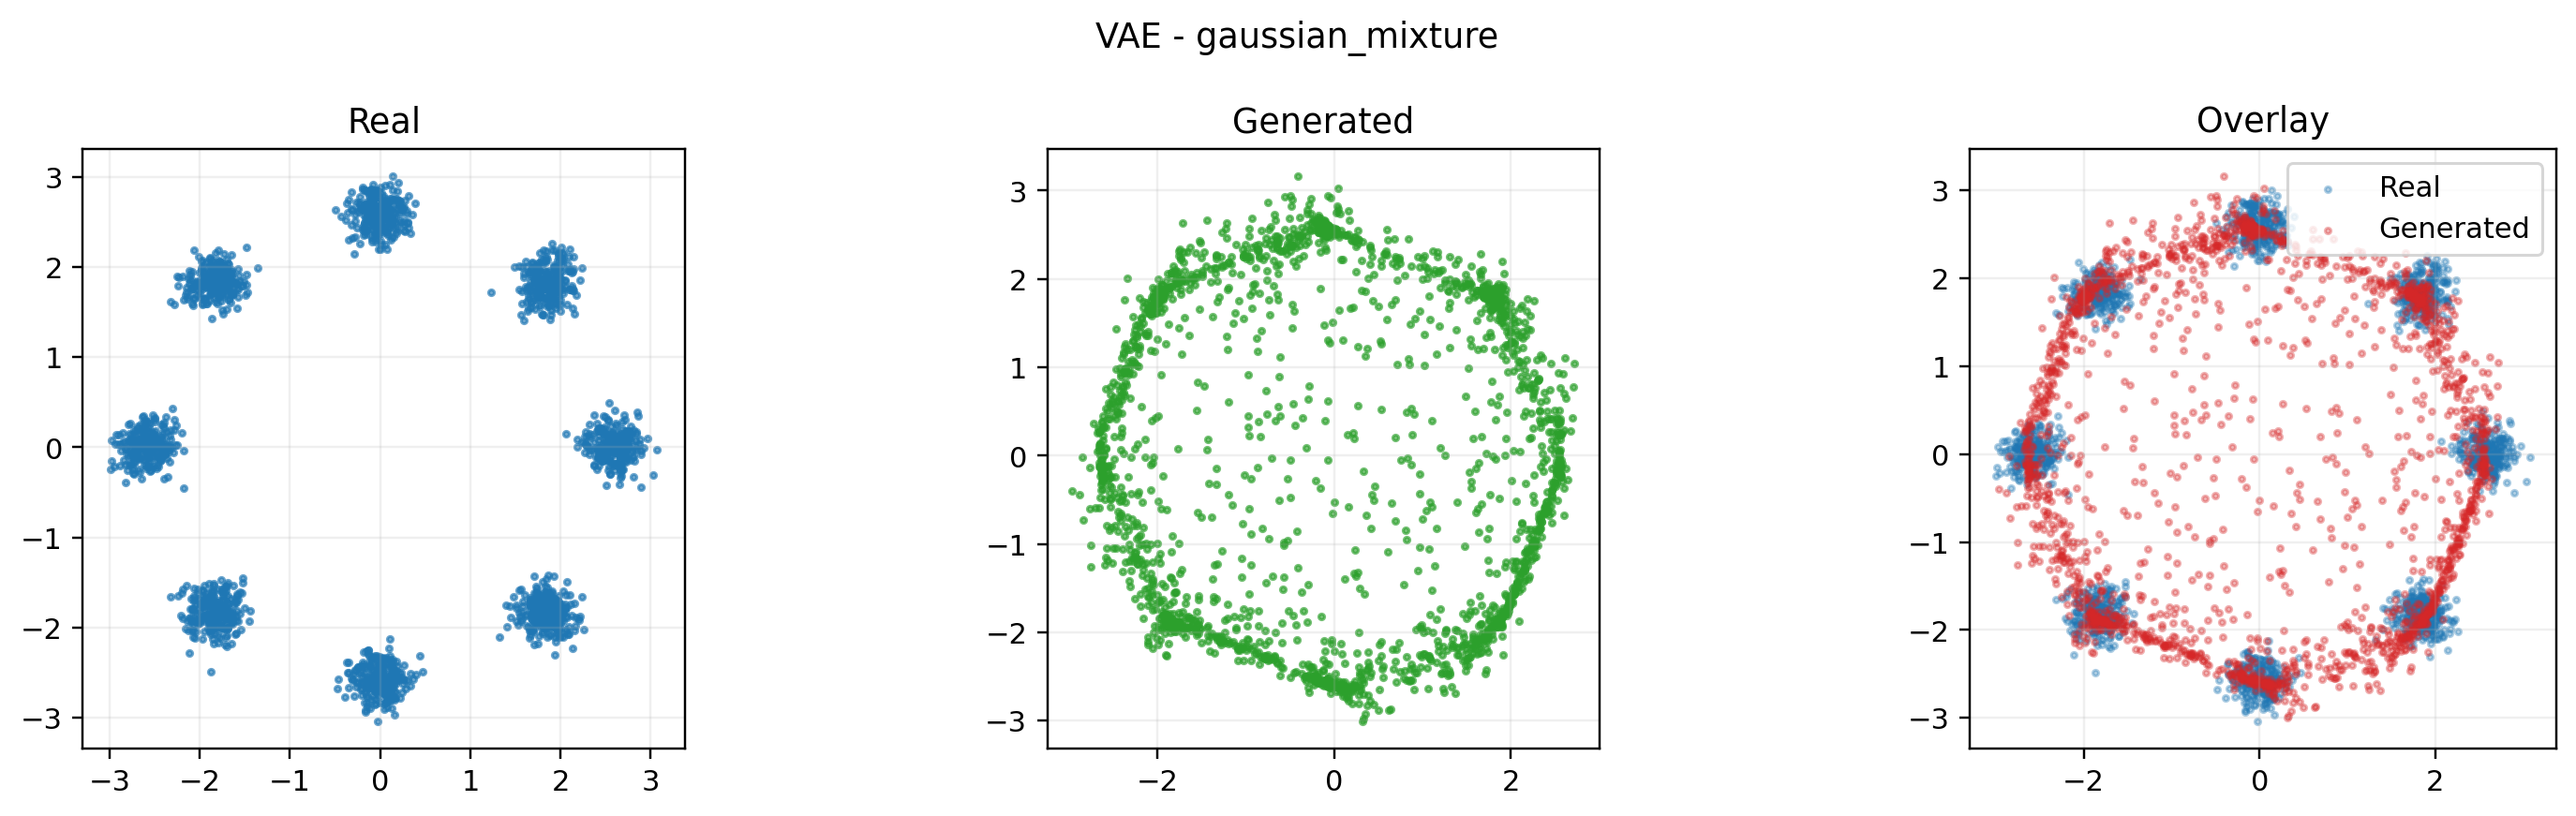
\includegraphics[width=\linewidth]{../outputs/figures/vae_gaussian_mixture_samples.png}
    \caption{VAE on Gaussian Mixture}
  \end{subfigure}
  \hfill
  \begin{subfigure}[b]{0.48\textwidth}
    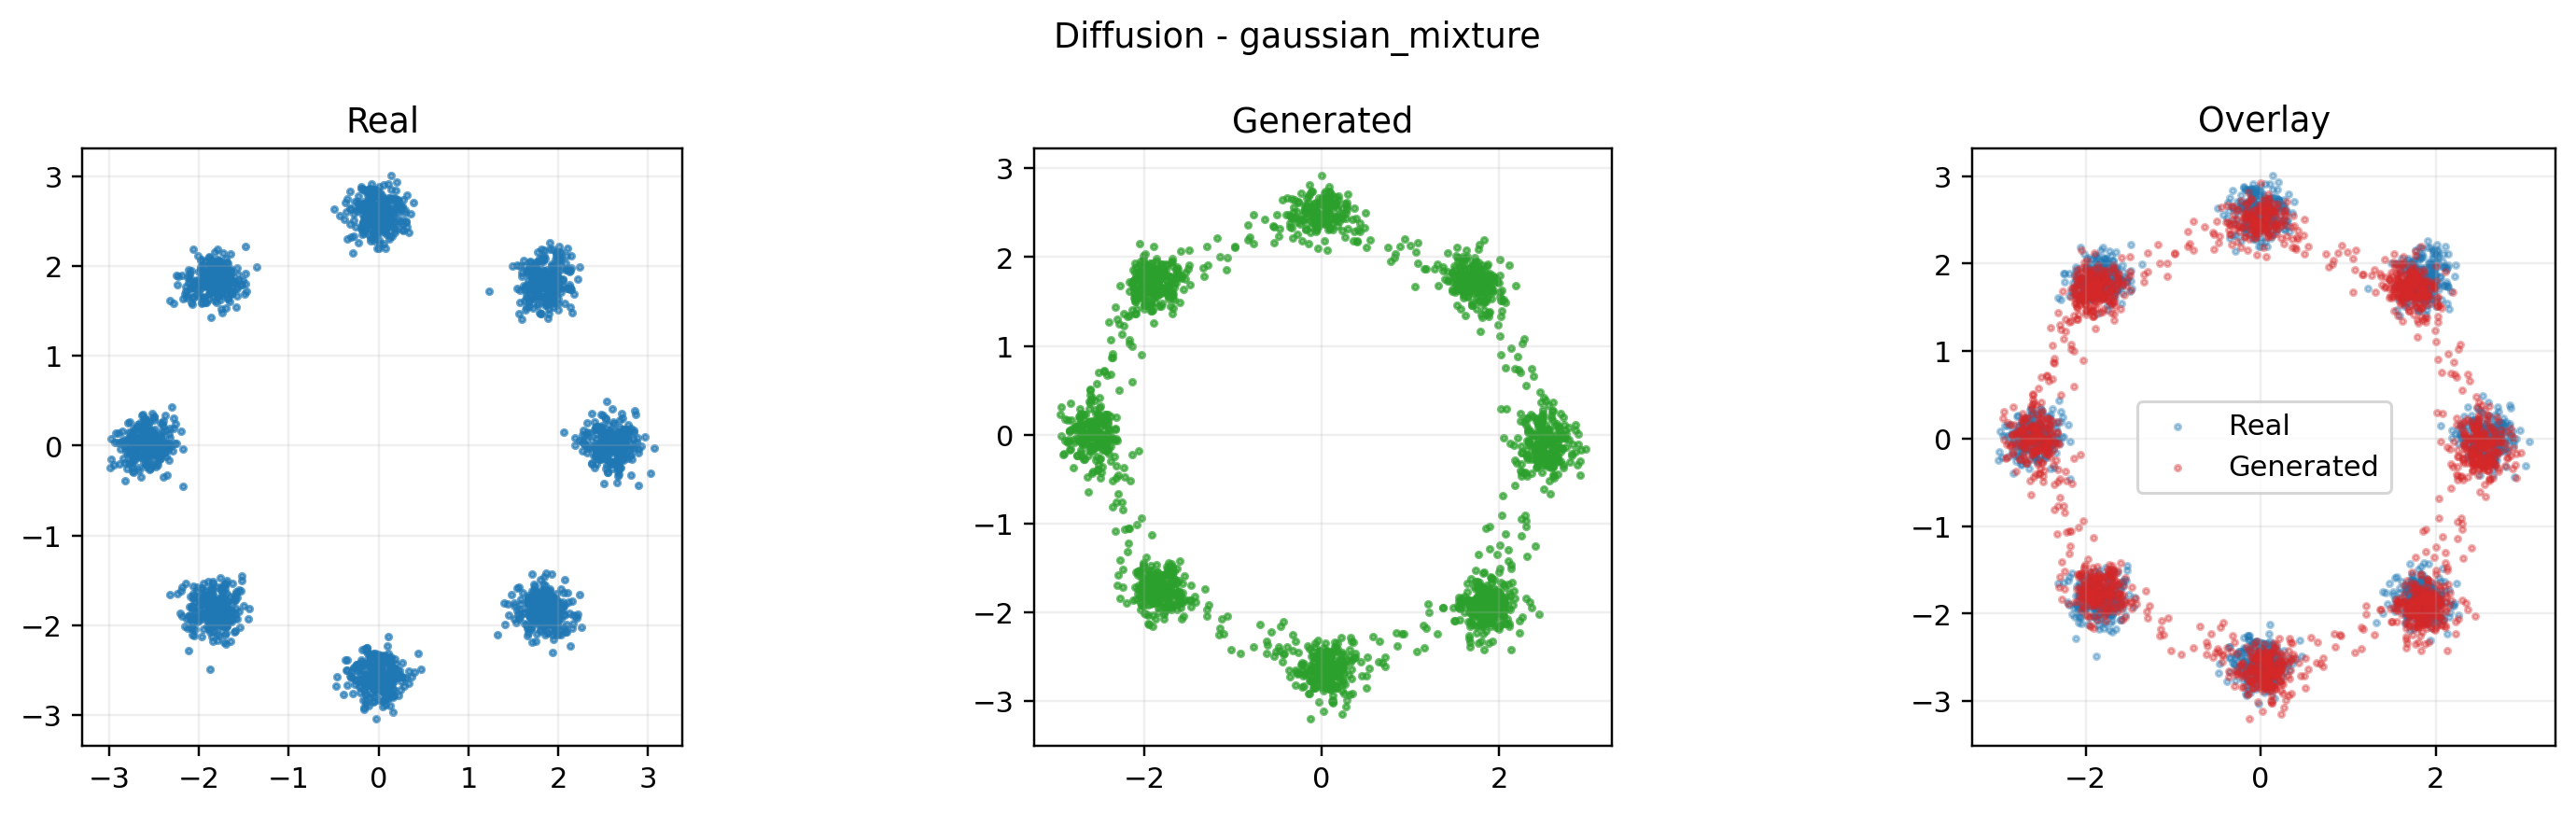
\includegraphics[width=\linewidth]{../outputs/figures/diffusion_gaussian_mixture_samples.png}
    \caption{Diffusion on Gaussian Mixture}
  \end{subfigure}
  \vspace{0.6em}
  \begin{subfigure}[b]{0.48\textwidth}
    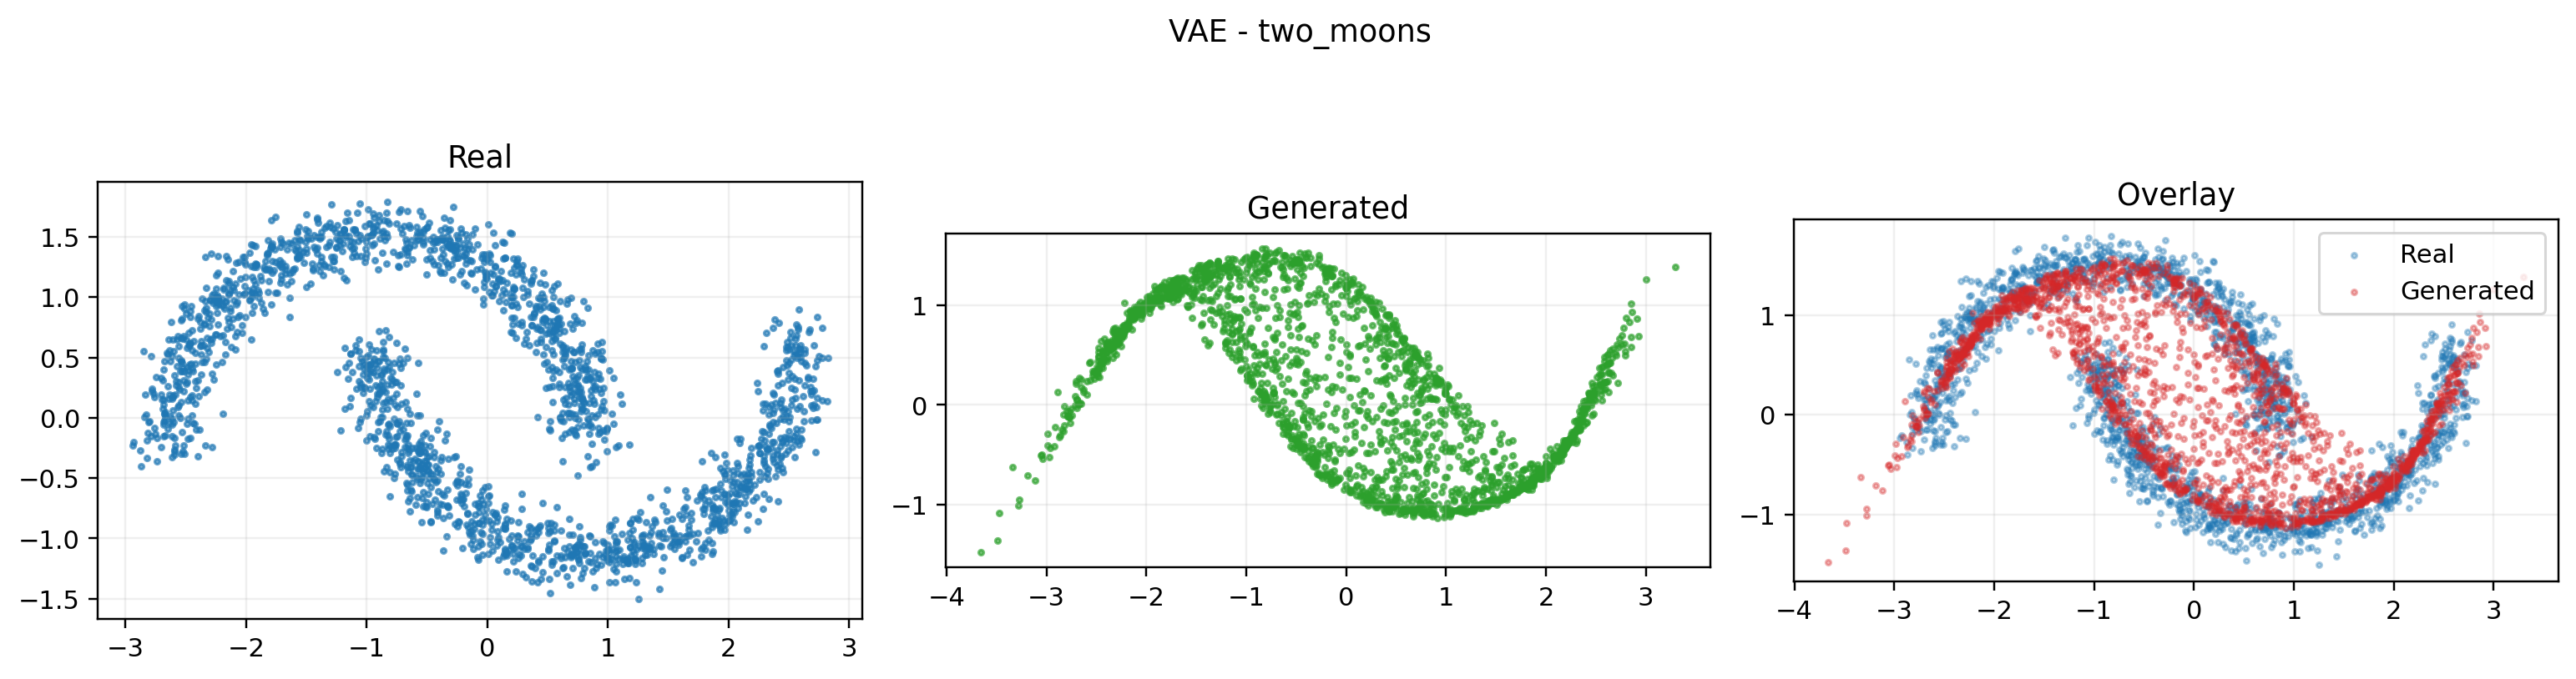
\includegraphics[width=\linewidth]{../outputs/figures/vae_two_moons_samples.png}
    \caption{VAE on Two Moons}
  \end{subfigure}
  \hfill
  \begin{subfigure}[b]{0.48\textwidth}
    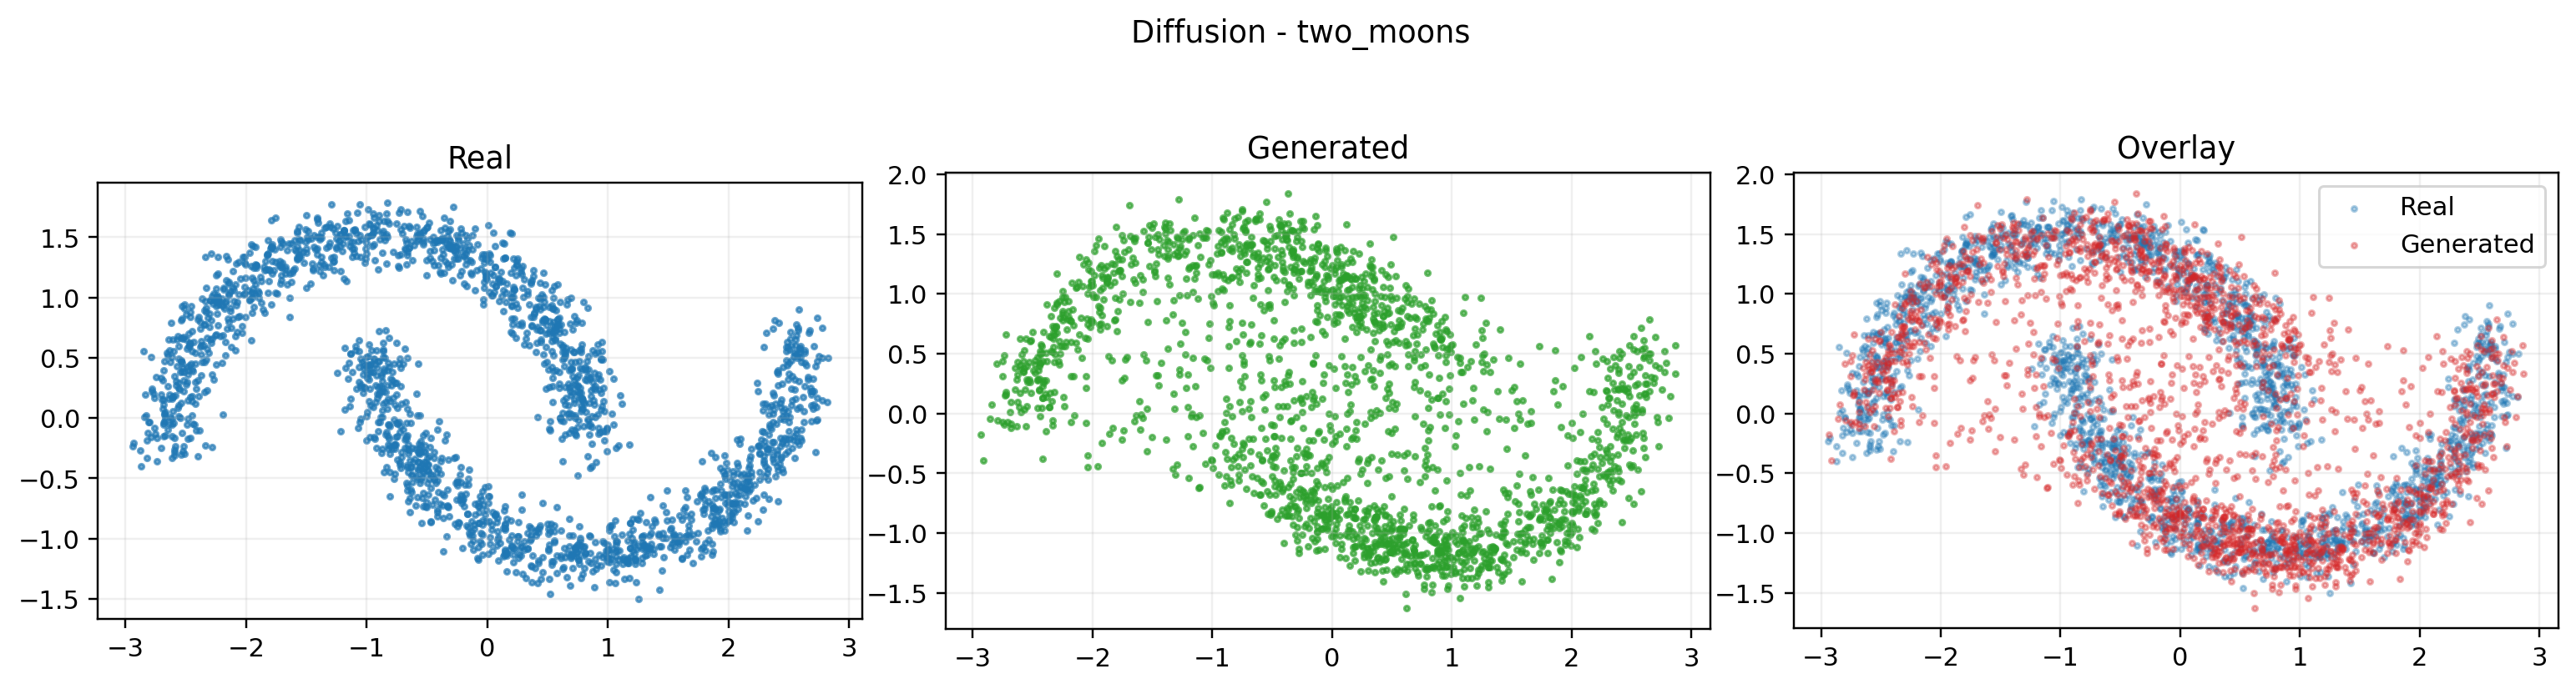
\includegraphics[width=\linewidth]{../outputs/figures/diffusion_two_moons_samples.png}
    \caption{Diffusion on Two Moons}
  \end{subfigure}
  \caption{Gaussian Mixture 与 Two Moons 上的生成样本对比。}
\end{figure}

在 Gaussian Mixture 上，Diffusion 更容易恢复多个局部簇的边界和均匀密度，而 VAE 对个别模态之间的间隙保持不够锐利；在 Two Moons 上，两者都能较好恢复双月形态，但 VAE 的局部贴合略好于 Diffusion，这与主实验表中的 MMD 结果相互印证。

\subsection{Diffusion 去噪过程可视化}

\begin{figure}[H]
  \centering
  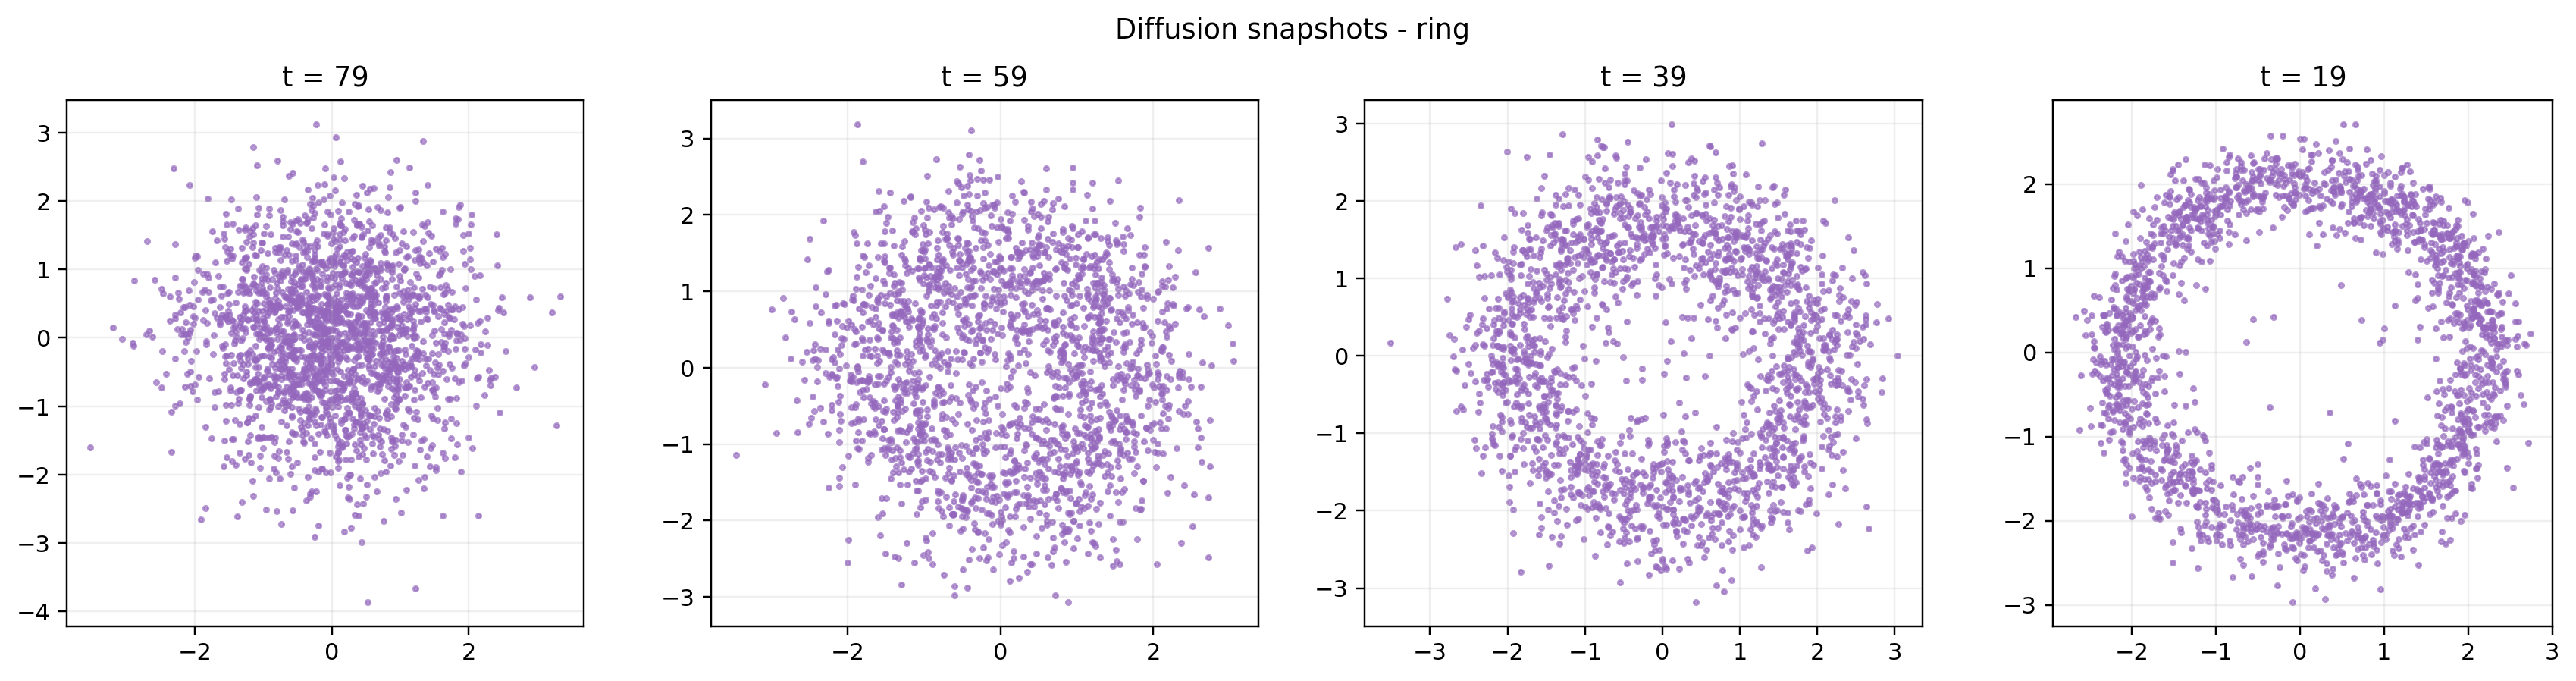
\includegraphics[width=0.88\textwidth]{../outputs/figures/diffusion_ring_snapshots.png}
  \caption{Ring 分布上的 Diffusion 采样过程快照。样本从近似高斯噪声逐步收缩并形成环状结构。}
\end{figure}

图中展示了扩散模型“从无序到有序”的典型生成路径：在早期阶段，样本呈现近似各向同性的高斯分布；中期开始出现环带轮廓；后期则逐步细化为清晰闭合的环形结构。该过程说明，Diffusion Model 的优势来自将复杂生成任务拆解为多个局部、可学习的去噪子任务。

\subsection{消融实验}

\begin{table}[H]
  \centering
  \caption{Spiral 分布上 VAE 的 KL 权重消融实验。}
  \begin{tabular}{lccc}
    \toprule
    设置 & MMD & SWD & 结论 \\
    \midrule
    $\beta=0.1$ & 0.0006 & 0.0719 & 最佳，重构优先 \\
    $\beta=0.5$ & 0.0015 & 0.0747 & 主实验设置 \\
    $\beta=1.0$ & 0.0032 & 0.0986 & 过强正则，性能下降 \\
    \bottomrule
  \end{tabular}
\end{table}

\begin{table}[H]
  \centering
  \caption{Spiral 分布上 Diffusion 步数消融实验。}
  \begin{tabular}{lccc}
    \toprule
    设置 & MMD & SWD & 结论 \\
    \midrule
    $T=20$ & 0.0028 & 0.0956 & 去噪精度不足 \\
    $T=80$ & 0.0008 & 0.0683 & 主实验设置，质量显著更好 \\
    \bottomrule
  \end{tabular}
\end{table}

消融结果揭示出两类模型不同的控制变量。对于 VAE，KL 权重本质上控制了“重构能力”和“潜空间规整性”之间的平衡；对复杂分布而言，较小的 $\beta$ 能显著缓解过度正则带来的结构损失。对于 Diffusion Model，扩散步数则更像一项硬约束：步数过小会降低反向过程对真实轨迹的逼近精度，从而明显削弱生成质量。

\subsection{增强骨干网络与采样加速}

为了将“更强骨干网络”和“更快采样策略”从设想变为可检验结果，本文在基线两层 MLP 之外进一步引入带残差块的 MLP 骨干，并结合前述 Spiral 消融中更优的 $\beta=0.1$ 对主实验进行重跑。表 \ref{tab:enhanced-main} 汇总了增强版主实验结果，同时额外报告 Chamfer 与 KDE-NLL 两项指标。

\begin{table}[H]
  \centering
  \small
  \caption{增强骨干网络后的主实验结果。}
  \label{tab:enhanced-main}
  \begin{tabular}{llccccc}
    \toprule
    模型 & 数据集 & MMD & SWD & Chamfer & KDE-NLL & 采样时间/s \\
    \midrule
    Diffusion & Gaussian Mixture & 0.0013 & 0.1399 & 0.0396 & 4.8728 & 0.0656 \\
    VAE       & Gaussian Mixture & 0.0012 & 0.1470 & 0.0957 & 4.8507 & 0.0017 \\
    Diffusion & Ring             & 0.0004 & 0.0754 & 0.0482 & 4.5504 & 0.0911 \\
    VAE       & Ring             & 0.0007 & 0.0878 & 0.0785 & 4.5145 & 0.0006 \\
    Diffusion & Spiral           & 0.0014 & 0.0962 & 0.0971 & 3.6783 & 0.0514 \\
    VAE       & Spiral           & 0.0008 & 0.0771 & 0.0929 & 3.7182 & 0.0008 \\
    Diffusion & Two Moons        & 0.0046 & 0.1310 & 0.0484 & 3.7576 & 0.0487 \\
    VAE       & Two Moons        & 0.0012 & 0.0888 & 0.0738 & 3.7654 & 0.0005 \\
    \bottomrule
  \end{tabular}
\end{table}

结果显示，增强骨干网络显著提升了 VAE 的竞争力：它在 Gaussian Mixture、Spiral 与 Two Moons 上都取得了更低的 MMD，且在 Spiral 上由基线阶段的劣势转为明显领先。与此同时，Diffusion 仍在 Ring 上保持最优，并在 Chamfer 指标上普遍更低，说明其局部邻域贴合能力依旧较强。若按平均值比较，增强版 VAE 的平均 MMD 为 0.00097，低于 Diffusion 的 0.00195；但 Diffusion 的平均 Chamfer 为 0.0583，优于 VAE 的 0.0852。这说明“更强骨干”并未简单地让某一类模型全面胜出，而是放大了两类方法在全局统计拟合与局部几何贴合上的差异。

在扩散模型采样端，本文进一步比较了原始 DDPM 与 DDIM 加速采样。表 \ref{tab:ddim-compare} 给出了 Spiral 上的对照结果。

\begin{table}[H]
  \centering
  \caption{Spiral 上 DDPM 与 DDIM 的采样对比。}
  \label{tab:ddim-compare}
  \begin{tabular}{lcccc}
    \toprule
    采样器 & MMD & SWD & Chamfer & 采样时间/s \\
    \midrule
    DDPM ($T=80$) & 0.0014 & 0.0962 & 0.0971 & 0.0571 \\
    DDIM (20 steps) & 0.0028 & 0.1123 & 0.0934 & 0.0133 \\
    \bottomrule
  \end{tabular}
\end{table}

可以看到，DDIM 将采样时间缩短到原来的约 $23\%$，而 MMD 与 SWD 仅出现中等幅度劣化，Chamfer 几乎保持同一量级。对二维任务而言，这一结果表明：当目标是快速生成大量样本用于可视化或下游分析时，DDIM 提供了一个相当划算的速度—质量折中。

\subsection{条件生成实验}

在条件生成方向上，本文不仅保留了基线的 Conditional VAE（CVAE），还进一步实现了 Conditional Diffusion，使“统一模型多分布可控生成”的比较从单一条件 VAE 拓展为两类生成范式之间的对照。图 \ref{fig:cond-diff} 给出了 Conditional Diffusion 的代表性生成结果。

\begin{figure}[H]
  \centering
  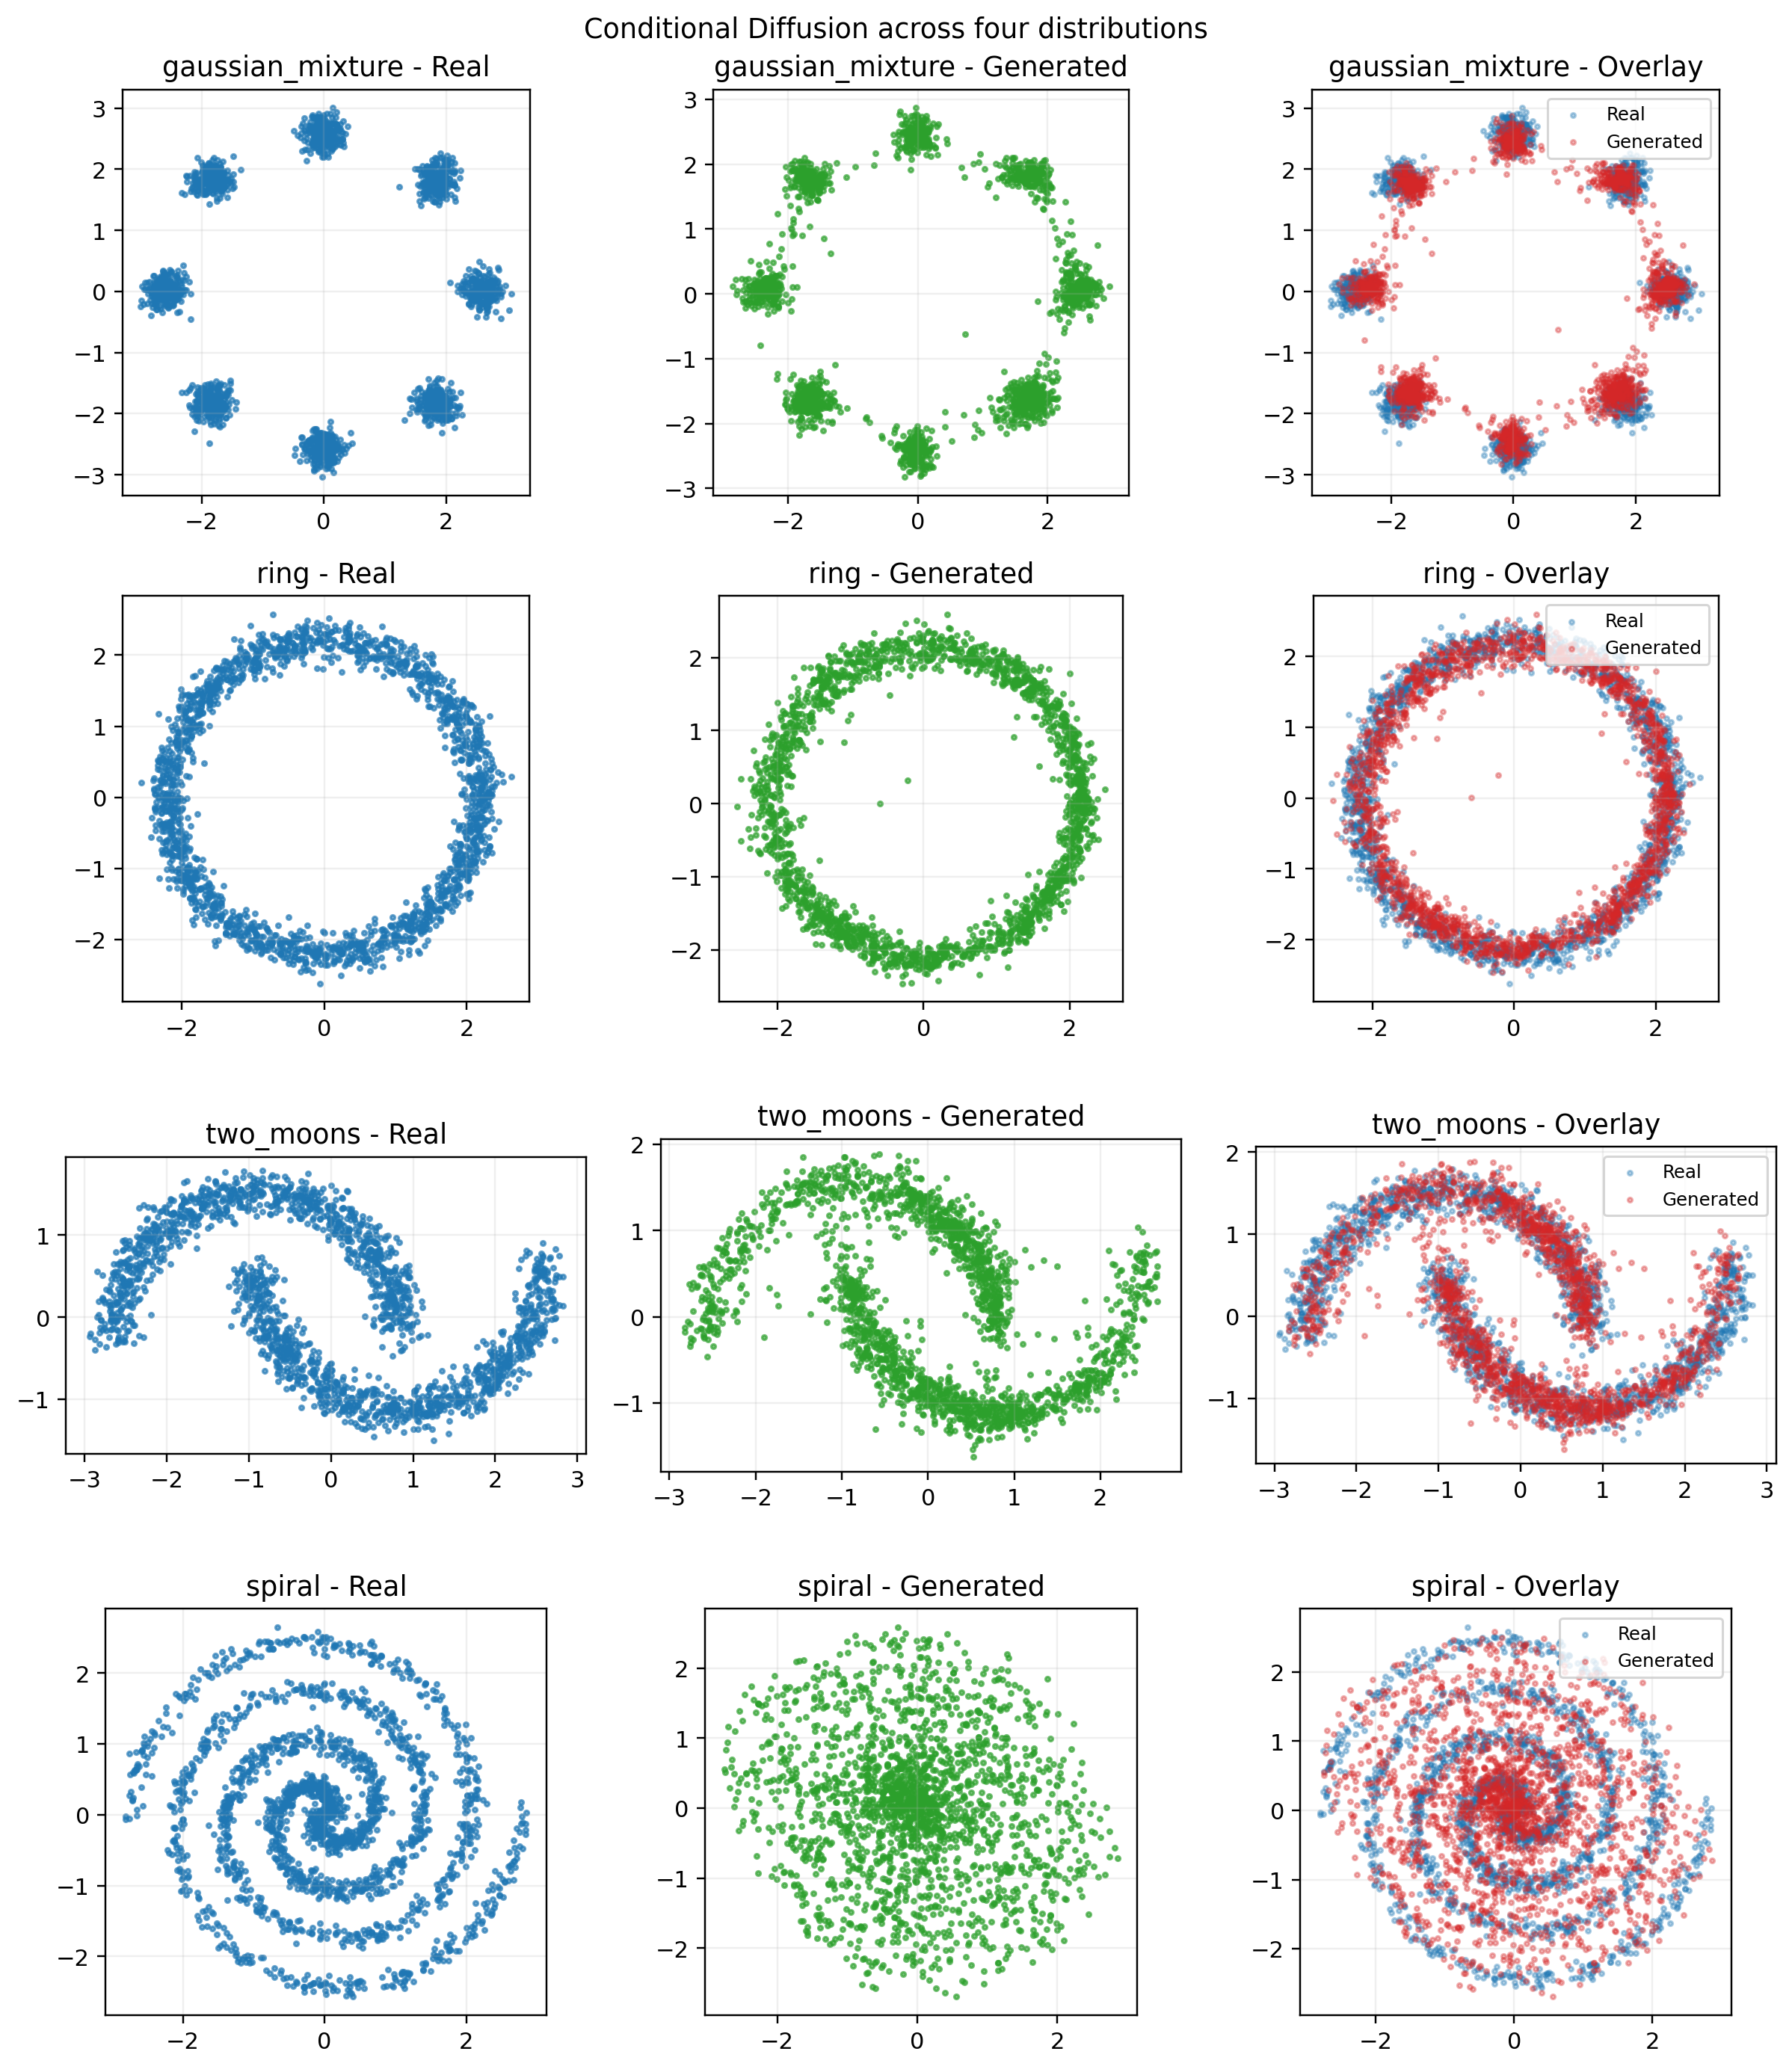
\includegraphics[width=0.94\textwidth]{../outputs/figures/optional/conditional_diffusion_samples.png}
  \caption{Conditional Diffusion 在四类分布上的条件生成结果。每一行对应一个条件标签，分别展示真实测试集、条件生成样本及叠加效果。}
  \label{fig:cond-diff}
\end{figure}

\begin{table}[H]
  \centering
  \caption{CVAE 与 Conditional Diffusion 的条件生成对比。}
  \begin{tabular}{lcccc}
    \toprule
    数据集 & CVAE MMD & CDiff MMD & CVAE SWD & CDiff SWD \\
    \midrule
    Gaussian Mixture & 0.0013 & 0.0019 & 0.1371 & 0.1629 \\
    Ring             & 0.0020 & 0.0011 & 0.1239 & 0.0915 \\
    Two Moons        & 0.0024 & 0.0122 & 0.0941 & 0.1927 \\
    Spiral           & 0.0031 & 0.0022 & 0.1268 & 0.0936 \\
    \bottomrule
  \end{tabular}
\end{table}

条件生成对照表明，两类条件模型各有偏好。CVAE 在 Gaussian Mixture 与 Two Moons 上更稳，平均 MMD 为 0.0022、平均 SWD 为 0.1205，且平均采样时间仅 0.0010\,s；Conditional Diffusion 则在 Ring 与 Spiral 上更优，平均 Chamfer 仅为 0.0611，显著低于 CVAE 的 0.0808，说明它在条件控制下仍更善于恢复连续几何结构。也就是说，当任务重点是高速、统一的条件采样时，CVAE 更具效率优势；当任务重点转向闭合流形或长程连续结构时，Conditional Diffusion 更值得采用。

\subsection{鲁棒性分析}

在鲁棒性方向上，本文不再局限于单一均匀离群点污染，而是进一步引入了三类污染：均匀离群点（uniform）、局部簇偏移（cluster shift）与异方差噪声（heteroscedastic）。同时，除 MMD 与 SWD 外，还增加 Chamfer 与 KDE-NLL 作为补充指标。表 \ref{tab:robustness-kinds} 汇总了 Ring 与 Spiral 上按污染类型平均后的结果。

\begin{table}[H]
  \centering
  \small
  \caption{不同污染类型下的鲁棒性分组结果（对 0\%、5\%、10\% 三种污染比例取平均）。}
  \label{tab:robustness-kinds}
  \begin{tabular}{lllccc}
    \toprule
    数据集 & 污染类型 & 模型 & MMD & SWD & Chamfer \\
    \midrule
    Ring & Uniform & Diffusion & 0.0016 & 0.1170 & 0.0838 \\
    Ring & Uniform & VAE       & 0.0010 & 0.1114 & 0.0992 \\
    Ring & Cluster Shift & Diffusion & 0.0022 & 0.1294 & 0.0886 \\
    Ring & Cluster Shift & VAE       & 0.0020 & 0.1305 & 0.0878 \\
    Ring & Heteroscedastic & Diffusion & 0.0019 & 0.1196 & 0.0825 \\
    Ring & Heteroscedastic & VAE       & 0.0012 & 0.1073 & 0.0807 \\
    Spiral & Uniform & Diffusion & 0.0010 & 0.0860 & 0.1040 \\
    Spiral & Uniform & VAE       & 0.0011 & 0.0836 & 0.1023 \\
    Spiral & Cluster Shift & Diffusion & 0.0012 & 0.0837 & 0.0973 \\
    Spiral & Cluster Shift & VAE       & 0.0015 & 0.0848 & 0.0911 \\
    Spiral & Heteroscedastic & Diffusion & 0.0012 & 0.0835 & 0.0980 \\
    Spiral & Heteroscedastic & VAE       & 0.0016 & 0.0854 & 0.0902 \\
    \bottomrule
  \end{tabular}
\end{table}

这组结果说明，污染类型与底层几何结构之间存在明显交互。在 Ring 上，局部簇偏移是最具破坏性的污染形式，因为它直接打断了窄环带的几何连续性；此时两类模型的 MMD 与 SWD 都明显高于 uniform 与 heteroscedastic 情况。对于 Spiral，Diffusion 在三类污染下都保持了更低的平均 MMD（约 0.0010--0.0012），说明其逐步去噪机制对全局分布形状更稳；但 VAE 在 SWD 与 Chamfer 上并不总是落后，尤其在 uniform 情况下还略低于 Diffusion，表明显式潜变量模型在局部平滑结构上的退化并不必然严重。总体而言，多类型污染实验比单一离群点测试更清楚地揭示了一个事实：鲁棒性并非“某个模型天生更抗噪”，而是取决于污染方式是否与目标流形的关键几何结构发生冲突。

\subsection{高维提升实验}

为检验二维结论在更复杂输入空间中的稳定性，本文进一步将原始二维样本通过多项式与三角基函数提升到 8 维，形成 lifted 高维基准。表 \ref{tab:highdim} 给出了 Gaussian Mixture 与 Spiral 上的代表性结果。

\begin{table}[H]
  \centering
  \caption{8 维 lifted 数据上的生成结果。}
  \label{tab:highdim}
  \begin{tabular}{llcccc}
    \toprule
    数据集 & 模型 & MMD & SWD & Chamfer & Mode Cov. \\
    \midrule
    Gaussian Mixture-8D & VAE       & 0.0043 & 0.2234 & 0.4821 & 1.00 \\
    Gaussian Mixture-8D & Diffusion & 0.0467 & 0.5773 & 0.5777 & 1.00 \\
    Spiral-8D           & VAE       & 0.0032 & 0.1106 & 0.4124 & 1.00 \\
    Spiral-8D           & Diffusion & 0.0988 & 0.5443 & 0.4395 & 1.00 \\
    \bottomrule
  \end{tabular}
\end{table}

高维 lifted 实验带来了两个重要信息。首先，二维场景中“Diffusion 在复杂几何上更优”的经验并不能直接外推到高维轻量设定；在当前 8 维实验中，VAE 保持了更稳定的 MMD 与 SWD，而 Diffusion 对模型容量与噪声调度更为敏感。其次，这一现象并不意味着扩散范式不适用于高维，而是表明：当输入维度升高后，噪声调度、时间条件网络与采样预算会更直接地影响最终生成质量。因此，高维验证不仅完成了更高维任务下的交叉检验，也进一步说明不同生成范式在容量分配与优化路径上存在系统差异。

\subsection{隐藏测试验证与高维扩散增强}

为检验主结论在未见样本与更强高维设定下的稳定性，本文补充开展了两组实验。第一组实验使用官方隐藏测试集作为未参与训练和调参的额外验证集，用于考察主要结论在 unseen split 上是否保持一致；第二组实验则在 8 维 lifted 场景中为 Diffusion 引入 cosine 噪声调度和更强的时间条件 MLP，以评估高维性能对模型设定的敏感性。表 \ref{tab:hidden-main} 与表 \ref{tab:highdim-upgrade} 分别给出对应结果。

\begin{table}[H]
  \centering
  \small
  \caption{主模型在隐藏测试集上的验证结果。}
  \label{tab:hidden-main}
  \begin{tabular}{llcccc}
    \toprule
    模型 & 数据集 & MMD & SWD & Chamfer & GMM-NLL \\
    \midrule
    VAE & Gaussian Mixture & 0.0007 & 0.1266 & 0.0929 & 2.6494 \\
    Diffusion & Gaussian Mixture & 0.0018 & 0.1471 & 0.0410 & 2.2115 \\
    VAE & Ring & 0.0011 & 0.0993 & 0.0860 & 2.6556 \\
    Diffusion & Ring & 0.0005 & 0.0829 & 0.0489 & 2.4747 \\
    VAE & Two Moons & 0.0016 & 0.0978 & 0.0668 & 2.6465 \\
    Diffusion & Two Moons & 0.0065 & 0.1457 & 0.0468 & 2.2643 \\
    VAE & Spiral & 0.0002 & 0.0690 & 0.0909 & 3.0968 \\
    Diffusion & Spiral & 0.0023 & 0.1183 & 0.0941 & 3.1110 \\
    \bottomrule
  \end{tabular}
\end{table}

隐藏测试结果表明，主文中的结论在未见样本上总体保持稳定：VAE 依旧在 Gaussian Mixture、Two Moons 与 Spiral 上取得更低的 MMD，而 Diffusion 继续在 Ring 上保持优势。值得注意的是，GMM-NLL 这一更严格的似然近似指标并不总与 MMD 完全一致，例如在 Gaussian Mixture 和 Two Moons 上，Diffusion 的 GMM-NLL 更低，但 MMD 与 SWD 反而更差；这说明概率密度代理与几何一致性指标捕捉的是不同侧面的生成质量，因此二者联合使用更具解释力。

\begin{table}[H]
  \centering
  \small
  \caption{高维 Diffusion 增强前后的对比。基线为线性噪声调度，改进版为 cosine 调度 + 时间条件 MLP。}
  \label{tab:highdim-upgrade}
  \begin{tabular}{lcccc}
    \toprule
    数据集 & 指标 & 基线 Diffusion & 改进 Diffusion & 改进幅度 \\
    \midrule
    Gaussian Mixture-8D & MMD & 0.0528 & 0.0014 & $\downarrow 97.4\%$ \\
    Gaussian Mixture-8D & SWD & 0.5999 & 0.1295 & $\downarrow 78.4\%$ \\
    Gaussian Mixture-8D & Chamfer & 0.6742 & 0.2169 & $\downarrow 67.8\%$ \\
    Spiral-8D & MMD & 0.0948 & 0.0128 & $\downarrow 86.5\%$ \\
    Spiral-8D & SWD & 0.5280 & 0.2683 & $\downarrow 49.2\%$ \\
    Spiral-8D & Chamfer & 0.4153 & 0.3390 & $\downarrow 18.4\%$ \\
    \bottomrule
  \end{tabular}
\end{table}

增强结果说明，高维 Diffusion 的性能对模型设定具有较强可塑性。引入 cosine 噪声调度和更强时间条件网络后，Gaussian Mixture-8D 上的 MMD 从 0.0528 显著降至 0.0014，Spiral-8D 上也从 0.0948 降至 0.0128；SWD 与 Chamfer 同样有明显下降。这表明此前观察到的高维差异中，有相当一部分来自噪声调度与条件网络表达能力。进一步结合表 \ref{tab:hidden-main} 与表 \ref{tab:highdim-upgrade} 可以看到，本文关于两类模型“简单分布与复杂流形表现不同、速度与质量权衡不同”的总体结论，在扩展设定下仍保持一致。

\subsection{综合讨论与方法反思}

结合主实验、骨干增强、采样加速、条件生成、鲁棒性与高维验证，可以对这一问题形成更完整的认识。
\begin{enumerate}
  \item \textbf{关于模型能力边界：}VAE 更适合结构相对清晰、需要高效采样的场景；Diffusion 更适合追求几何保真度和复杂拓扑拟合的场景。
  \item \textbf{关于扩展实验的价值：}条件生成实验表明，模型差异并不限于无条件采样阶段，而会进一步体现在条件控制下的几何恢复能力；鲁棒性实验则说明，模型表现会随着污染方式与底层流形结构的相互作用而系统变化。
  \item \textbf{关于实验结论的稳定性：}隐藏测试验证、高维扩展与多指标交叉比较共同表明，正文中的主要结论并非来自单次跑分，而是在多组对照实验中反复出现的稳定现象。
\end{enumerate}

\subsection{结果说明}

结合主实验、条件生成、鲁棒性测试、隐藏测试验证以及高维 lifted 扩展实验，本文已经形成一套闭环的经验比较结果。不同结论并非来自单一指标或单一数据划分，而是在 MMD、SWD、Chamfer、KDE-NLL、GMM-NLL、Mode Coverage 以及采样时间等多个维度上相互印证。整体来看，VAE 在训练稳定性与采样效率上保持明显优势，并在 Gaussian Mixture、Two Moons 等结构相对规则的数据上取得了更稳健的分布拟合结果；Diffusion 则在 Ring、Spiral 等更强调连续几何结构的数据上表现出更强的样本几何恢复能力。隐藏测试与高维扩展进一步表明，这种差异具有一致性，也说明两类模型在二维几何数据生成任务中各自对应着清晰而稳定的适用场景。

\section{总结与讨论}

\subsection{主要结论}

本文围绕二维生成建模任务，系统比较了 VAE 与 Diffusion Model 两类深度生成方法，并得到以下结论：
\begin{enumerate}
  \item 在基线轻量设置下，Diffusion 在 Ring 等闭合流形上优势明显；在引入残差骨干并重新调优后，VAE 在 Gaussian Mixture、Two Moons 与 Spiral 上取得了更低的 MMD；
  \item VAE 的关键调节量是 KL 权重，Diffusion 的关键调节量是扩散步数，两者的超参数敏感性来源不同；
  \item DDIM 在 Spiral 上将扩散采样时间从 0.0571\,s 降至 0.0133\,s，代价是 MMD 与 SWD 有一定上升，体现了可观的速度—质量折中；
  \item 条件生成实验表明，CVAE 的平均 MMD 和平均采样速度更优，而 Conditional Diffusion 在 Ring 与 Spiral 上具有更好的条件几何保真度；
  \item 多类型污染实验说明，Ring 对局部簇偏移最敏感，而 Spiral 上 Diffusion 在三类污染下都保持了更低的平均 MMD；
  \item 隐藏测试验证表明，主文结论在未见样本上总体稳定：VAE 仍在 Gaussian Mixture、Two Moons 与 Spiral 上更强，而 Diffusion 继续在 Ring 上占优；
  \item 在 8 维 lifted 场景中，cosine 调度与更强时间条件网络可显著改善 Diffusion 的高维表现，说明高维结果对噪声调度与条件网络容量较为敏感。
\end{enumerate}

\subsection{两类模型差异的机理讨论}

VAE 与 Diffusion Model 的差异并非偶然，而是源于生成路径与优化目标的本质不同。VAE 在单次前向传播中完成从潜变量到样本的整体映射，因此解码器必须同时承担全局结构与局部细节的恢复任务；而 Diffusion Model 将这一任务分解为多个局部去噪步骤，使得每一步的学习难度更低，也更容易维持复杂流形的连续性。另一方面，VAE 显式维护低维潜空间，具有更好的解释性与快速采样能力；Diffusion 则以更高的计算代价换取更强的表示容量与更高的样本精度。

进一步地，增强骨干、条件扩散、多类型污染与高维验证共同强化了这一认识。残差骨干使 VAE 的整体表达能力明显提升，说明显式潜变量模型的“上限”很大程度上受限于解码器容量；而 DDIM 与 Conditional Diffusion 的结果则表明，扩散范式可以通过更灵活的采样策略和条件控制保持几何优势，但这种优势在高维轻量设定下并不会自动保留。因而，两类模型并不是简单的“谁更新谁就更强”，而是受到骨干容量、采样预算、任务几何结构与目标维度共同决定的。


\clearpage
\bibliographystyle{gbt7714-numerical}
\bibliography{references}

\appendix

\section{补充实验说明}

为保证主文中的比较具有可解释性，附录中的扩展实验均遵循与主实验一致的原则：四类分布使用相同的数据划分方式，VAE、Diffusion 与条件生成模型采用统一的训练流程与评价指标，所有结果均在相同硬件环境下重复得到。这样处理的目的在于尽量把性能差异归因于模型机制本身，而不是归因于实验设置不一致。

附录所列结果主要承担两项作用。其一是补充正文中未完全展开的数值细节，例如条件生成在各分布上的分项表现，以及不同污染比例下鲁棒性指标的变化；其二是帮助验证主文结论在不同骨干、采样策略、污染类型与维度设定下会发生怎样的变化，从而使全文分析更完整、更可追溯。

\section{扩展实验补充表}

\begin{table}[H]
  \centering
  \caption{Conditional VAE 的完整分布别结果。}
  \begin{tabular}{lccccc}
    \toprule
    数据集 & MMD & SWD & Mode Cov. & 训练时间/s & 采样时间/s \\
    \midrule
    Gaussian Mixture & 0.0015 & 0.1718 & 1.00 & 13.6230 & 0.0012 \\
    Ring             & 0.0016 & 0.1122 & 1.00 & 13.6230 & 0.0007 \\
    Two Moons        & 0.0014 & 0.0904 & 1.00 & 13.6230 & 0.0006 \\
    Spiral           & 0.0013 & 0.0758 & 1.00 & 13.6230 & 0.0006 \\
    \bottomrule
  \end{tabular}
\end{table}

\begin{table}[H]
  \centering
  \caption{Ring 与 Spiral 上的鲁棒性实验完整结果汇总。}
  \small
  \begin{tabular}{llcccc}
    \toprule
    数据集 & 模型 & 污染比例 & MMD & SWD & 采样时间/s \\
    \midrule
    Ring & VAE & 0.00 & 0.0016 & 0.1133 & 0.0011 \\
    Ring & VAE & 0.05 & 0.0018 & 0.1332 & 0.0003 \\
    Ring & VAE & 0.10 & 0.0009 & 0.1211 & 0.0003 \\
    Ring & Diffusion & 0.00 & 0.0011 & 0.0875 & 0.0409 \\
    Ring & Diffusion & 0.05 & 0.0003 & 0.0664 & 0.0355 \\
    Ring & Diffusion & 0.10 & 0.0003 & 0.0621 & 0.0443 \\
    Spiral & VAE & 0.00 & 0.0026 & 0.1010 & 0.0002 \\
    Spiral & VAE & 0.05 & 0.0016 & 0.0992 & 0.0003 \\
    Spiral & VAE & 0.10 & 0.0020 & 0.1152 & 0.0004 \\
    Spiral & Diffusion & 0.00 & 0.0011 & 0.0756 & 0.0324 \\
    Spiral & Diffusion & 0.05 & 0.0018 & 0.1026 & 0.0385 \\
    Spiral & Diffusion & 0.10 & 0.0011 & 0.0874 & 0.0325 \\
    \bottomrule
  \end{tabular}
\end{table}

\begin{table}[H]
  \centering
  \caption{四类测试集的补充统计量。}
  \small
  \begin{tabular}{lcccccc}
    \toprule
    数据集 & $\mu_x$ & $\mu_y$ & $\sigma_x$ & $\sigma_y$ & 平均半径 & 协方差迹 \\
    \midrule
    Gaussian Mixture & 0.036 & 0.014 & 1.838 & 1.838 & 2.595 & 6.762 \\
    Ring             & -0.029 & -0.025 & 1.572 & 1.546 & 2.201 & 4.862 \\
    Two Moons        & -0.040 & 0.189 & 1.496 & 0.873 & 1.606 & 3.003 \\
    Spiral           & 0.028 & -0.006 & 1.162 & 1.138 & 1.427 & 2.648 \\
    \bottomrule
  \end{tabular}
\end{table}

\end{document}
